\documentclass[12pt, notitlepage]{article} 

%\usepackage{graphicx,float,wrapfig}
\usepackage[margin=1in]{geometry}
\usepackage{enumerate}
\usepackage{multirow}
\usepackage{empheq}
\usepackage{indentfirst}
\usepackage{natbib}

\usepackage[pdftex]{graphicx}
\usepackage{setspace}
\usepackage{hyperref}

\usepackage{color}
\usepackage{comment}

\usepackage{amsmath,amssymb,amstext, bm} 

\usepackage{setspace}
%\doublespacing
\setstretch{1.8}

%\usepackage{lineno}
%\linenumbers

\DeclareMathOperator{\Tr}{Tr}
\newcommand{\var}{\mathrm{var}}
\newcommand{\corr}{\mathrm{corr}}

\title{A Bivariate Semiparametric Stochastic Mixed Effects Model}
%\author{Kexin Ji \& Joel A. Dubin}
\date{}



\begin{document}

\maketitle


\begin{abstract}
We propose and consider inference for a semiparametric stochastic mixed effects model for bivariate periodic repeated measures data.  The bivariate model uses parametric fixed effects for modeling covariate effects and periodic smooth nonparametric functions for each of the two underlying time effects. The between-subject and within-subject correlations are modelled using separate but correlated random effects and a bivariate Gaussian random field, respectively. We derive estimators for both the fixed effects regression coefficients and the nonparametric time functions using maximum penalized likelihood, where the resulting estimator for the nonparametric time function is a smoothing spline. The smoothing parameters and all variance components are estimated simultaneously using restricted maximum likelihood.  Simulation results show that the parameter estimates are close to the true values with small standard errors. We demonstrate the proposed methodology on a real longitudinal dataset of pre-menopausal women.

\vspace{5mm}
\noindent KEYWORDS: Bivariate longitudinal data; Cyclic; Gaussian field; Penalized likelihood; Smoothing spline.
\end{abstract}


\thispagestyle{empty}
\clearpage
\setcounter{page}{1}
%\begin{keyword}
%    Something else
%\end{keyword}

%======================================================================
%
% S.1 INTRODUCTION
%
%
%======================================================================
\section{Introduction}


Longitudinal data analysis has wide applications in areas such as medicine and agriculture. 
One distinctive feature of longitudinal data is that measurements of each subject are collected repeatedly over time; thus, each measurement for the same subject is no longer independent.  This induces a correlation structure that needs to be modeled carefully. Many methods have been developed over the years to accommodate this additional structure, e.g., \cite{Laird:1982}, \cite{Liang:1986}. 

Beyond these earlier proposed models for linear and generalized linear longitudinal data, there have have been many extensions to allow for further flexibility in the mean, variance and/or correlation structure.  For example, 
\citet{Brumback:1998} used natural cubic splines to model the mean structure of the linear mixed model.  
They extended the traditional LME  model to generalized smoothing spline models for samples of curves stratified by nested and crossed factors and specified the design matrices associated with fixed effects and random effects by bases of functions, as opposed to the usual known covariates matrices.  \citet{Verb:Cull:Kenw:Welh:quan:1999} advocated a similar approach as \citet{Brumback:1998}, where data-based determination of the smoothing parameters was advocated, yet their model specification is slightly different; and the techniques were applied to the analysis of designed experiments. 

\citet*{Tayl:Cumb:Sy:quan:1994} used a particular stochastic process to model longitudinal data in addition to the usual random effect term which  induces within-subject correlation. \cite {Zhang:1998} combined both the smoothing spline to measure mean structure and  various stationary and nonstationary stochastic processes to model serial correlation into one cohesive model. To further model cyclic responses, 
\citet*{Zhan:Lin:Sowe:quan:2000} 
extended their previous work and proposed a  semiparametric stochastic mixed model for periodic longitudinal data. They used parametric functions to model the covariate effects and a periodic smooth nonparametric function to model the underlying complex periodic time course. The within-subject covariance is modeled using a random intercept and a stochastic process with periodic variance function. Instead of cubic smoothing spline, \cite{Welh:Cull:Kenw:Thom:quan:2006} modelled cyclic longitudinal data using mixed model L-splines. 
%Meyer et al \cite{meyer} proposed a functional data analysis approach to model cyclic data. 
\citet{Wood:2006} modified penalized cubic regression spline to model a cyclic smooth function. 

All of the approaches mentioned above are to be applied on univariate longitudinal responses. A growing number of applications require techniques to model bivariate, and in more generality, multivariate responses. More recently, \cite{Raffa:2015} modeled bivariate longitudinal responses, from outcomes of different data types, via a mixed effects hidden Markov modeling approach.  And, most relevant in terms of the type of data focused in this paper,  \cite{Liu:Capp:Crof:Guo:quan:2014} extended the univariate state space model in time series analysis, and proposed a bivariate hierarchical state space model to bivariate circadian rhythmic  longitudinal responses. 
Each response is modelled by a hierarchical state space model, with both population-average and subject-specific components. The bivariate model is constructed by linking the univariate models based on the hypothesized relationship. \citet*{Sy:Cumb:Tayl:quan:1997} employed multivariate stochastic processes to jointly model  bivariate longitudinal data. 


We extend \citet {Zhang:1998} and \citet{Zhan:Lin:Sowe:quan:2000} and propose a bivariate semiparametric stochastic mixed model for bivariate periodic repeated measures data.  The bivariate model uses parametric fixed effects for modeling covariate effects and periodic smooth nonparametric functions for each of the two underlying time effects. In addition, the between-subject and within-subject correlations are modeled using separate but correlated random effects and a bivariate Gaussian random field, respectively. We derive maximum penalized likelihood estimators for both the fixed effects regression coefficients and the nonparametric time functions. The smoothing parameters and all variance components are estimated simultaneously using restricted maximum likelihood.  


The paper is organized as followed. Section \ref{modelSpe} specifies the proposed model with assumptions. Section \ref{est} provides estimation and inference procedures. Specifically, Sections \ref{MatrixNotation} and \ref{estimation} gives estimation procedures for  the model parameters, the nonparametric components, random effects and the Gaussian fields.  
Section \ref{biasCov} specifies the biases and covariances for all the estimators given in Section \ref{estimation}; and Section \ref{estSmoo}  concludes this section by providing the estimation procedures of the smoothing parameters and variance components. 
Section \ref{simulation} investigates the proposed methodology through a simulation study.  
Section \ref{dataAnalysis}  illustrates the model by analyzing bivariate longitudinal female hormone data collected daily over a single menstrual cycle, and finally, Section \ref{conclu} provides a summary of our proposed model, and discusses challenges and future work.


%======================================================================
%
% S.2 MODEL SPECIFICATION
%
%
%======================================================================

\section{The Bivariate Semiparametric Stochastic Mixed Effects Model} \label{modelSpe}


%---------------------------------------------------------------------------------------------------------------------------
\subsection{General Bivariate Longitudinal Model with Joint Distribution of Random Effects}
We propose a semiparametric stochastic bivariate mixed effects model, where the joint model assumes a semiparametric mixed effects model for each outcome. 
This is a clear and important extension of the \citet {Zhang:1998} and \citet{Zhan:Lin:Sowe:quan:2000} model. 
The univariate models for each outcome are connected  through the specification of the correlation structure for the random effects.
Denote $\{Y_{1ij}, Y_{2ij}\}$ to be the bivariate response for the $i$th subject at time point $j$, 
$i = 1, \dots, m$ and $j = 1, \dots, n_i$. 
The bivariate model is
\begin{eqnarray} \label{biv}
Y_{1ij} 
&=& 
\bm{X}_{1ij}^T\bm{\beta}_1 + f_1(t_{ij}) + \bm{Z}_{1ij}^T
\bm{b}_{1i} + 
U_{1i}(t_{ij}) + 
\epsilon_{1ij}
 \nonumber 
\\
Y_{2ij} 
&=& 
\bm X_{2ij}^T \bm \beta_2 + f_2(t_{ij}) + \bm Z_{2ij}^T
\bm b_{2i} + 
U_{2i}(t_{ij}) + \epsilon_{2ij}, 
\end{eqnarray}
where 
$(\bm X_{1ij}, \bm X_{2ij})$ are known covariates associated with the fixed effects; 
$(\bm Z_{1ij}$, $\bm Z_{2ij})$ are known covariates associated with the random effects; 
$\bm \beta_1$ and $\bm \beta_2$ are $p_1 \times 1$ and $p_2 \times 1$ vectors of regression coefficients, containing the fixed effects connected to each response,
 respectively; 
$\bm b_{1i}$ and $\bm b_{2i}$ are $q_1 \times 1$ and $q_2 \times 1$ vectors of random effects, respectively; 
$f_1(t)$ and $f_2(t)$ are  twice-differentiable periodic smooth functions of time with  periods $T_1$ and $T_2$, respectively; 
$\{(U_{1i}(t_{ij}), U_{2i}(t_{ij})), t_{ij} \in \{t_{i1}, \dots, t_{in_i}\}, i = 1, \dots, m, j = 1, \dots, n_i  \}$ is a mean zero bivariate Gaussian field  with 
covariance matrix 
%%\E\{((U_i(s))^\prime U_i(t)\} =
\begin{eqnarray*}
\boldsymbol C_i(s, t) &=&
%  \begin{pmatrix}
%  E[U_{i1}(s) U_{i1}(t)] &  E[U_{i1}(s) U_{i2}(t)]   \\
%E[U_{i2}(s) U_{i1}(t)]  &   E[U_{i2}(s) U_{i2}(t)]  
% \end{pmatrix} \\ 
%&=&
  \begin{pmatrix}
 \sqrt {\xi_1(s) \xi_1(t)} \eta_1(\rho_1; s, t) &   \sqrt {\xi_1(s) \xi_2(t)} \eta_3(\rho_3; s, t)
  \\
 \sqrt {\xi_2(s) \xi_1(t)} \eta_3(\rho_3; t, s)
 &   \sqrt {\xi_2(s) \xi_2(t)} \eta_2(\rho_2; s, t)
 \end{pmatrix}
\end{eqnarray*}
%$$
%C_{ij}(s, t) = \E\{((U_i(s))^\prime U_i(t)\}
%$$
%both mean-zero Gaussian processes with
where 
$\xi_1(t)$ and $\xi_2(t)$ are periodic variance functions;  
${\rm corr} (U_{1i}(t), U_{1i}(s)) = \eta_1(\rho_1; s, t)$,  \\
${\rm corr} (U_{2i}(t), U_{2i}(s)) = \eta_2(\rho_2; s, t)$, 
and ${\rm corr} (U_{1i}(t), U_{2i}(s)) = \eta_3(\rho_3; s, t)$
 are correlation functions, where $\rho_1 \in [0, 1]$,  $\rho_2 \in [0, 1]$ and $\rho_3 \in [0, 1]$ are correlation parameters; 
and 
the measurement errors $(\epsilon_{1ij}, \epsilon_{2ij})^T$ are bivariate  normal with mean $\bm 0$ and variance $  \begin{pmatrix}
  \sigma_1^2 &  \sigma_{12}^2  \\
\sigma_{12}^2 &   \sigma_2^2 
 \end{pmatrix}$.
%$$
% \begin{pmatrix}
%  {\epsilon_{1ij}}  \\
%{\epsilon_{2ij}} 
% \end{pmatrix}
% \sim 
% N_2 \left(
%\boldsymbol 0,
%  \begin{pmatrix}
%  \sigma_1^2 &  \sigma_{12}^2  \\
%\sigma_{12}^2 &   \sigma_2^2 
% \end{pmatrix}
% \right).
%$$
We assume that $\bm b_{ki}, k = 1, 2$ to be  $(q_1 + q_2)$-dimensional normal  with mean zero and covariance matrix $\boldsymbol D(\boldsymbol \phi)$.  
These random effects, $\bm b_{1i}$ and $\bm b_{2i}$, are assumed to be separate but correlated. 
Further, 
we assume that the random effects, the stochastic process and the measurement error to be mutually independent. 






Denote $\bm Y_{ij} = (Y_{1ij}, Y_{2ij})^T$ and similarly for $\bm \beta$, $\bm b_i$, $\bm f(t_{ij})$, $\bm U_i(t_{ij})$ and $\bm \epsilon_{ij}$, and let $\bm X_{ij} = {\rm diag} (\bm X_{1ij}^T, \bm X_{2ij}^T)$ and similarly for $\bm Z_{ij}$. 
%\[
%% Y_ij
% \boldsymbol Y_{ij} =
% \begin{pmatrix}
%   Y_{1ij}  \\
%  Y_{2ij}
% \end{pmatrix}
% \in {\rm I\!R}^{2}
% \]
% to be the response vector; 
%% $$
%% 
%% $$
%\[
%% X_ij
%\boldsymbol {X_{ij}}
%=
% \begin{pmatrix}
%  \boldsymbol {X_{1ij}}^T  &  \boldsymbol 0\\
% \boldsymbol 0 &  \boldsymbol {X_{2ij}}^T
% \end{pmatrix}
%  \in {\rm I\!R}^{(p_1+p_2) \times 2}, 
% % $$
%% 
%% $$
%\quad
% \boldsymbol \beta
% =
%  \begin{pmatrix}
%  \boldsymbol\beta_1 \\
%  \boldsymbol\beta_2
% \end{pmatrix}
%   \in {\rm I\!R}^{(p_1+p_2)},
% \]
% to be the matrix of known covariates and the vector of  regression coefficients respectively; 
%\[
%% Z_ij
%\boldsymbol{Z_{ij}}  =
% \begin{pmatrix}
%\boldsymbol {Z_{1ij}}^T & \boldsymbol 0 \\
%\boldsymbol 0 & \boldsymbol {Z_{2ij}}^T
% \end{pmatrix}
%   \in {\rm I\!R}^{(q_1+q_2) \times 2}, 
% % $$
%% 
%% $$
%\quad
%% b_i
%\boldsymbol b_i
%=
%  \begin{pmatrix}
%b_{1i} \\
%b_{2i}
% \end{pmatrix}
%    \in {\rm I\!R}^{(q_1+q_2)}, 
%    \]
% to be the matrix of known covariates associated with the random effects and the vector of random effects respectively; 
% and finally 
% \[
% % $$
%% 
%% $$
%\quad
%\boldsymbol f(t_{ij})
%=
%  \begin{pmatrix}
%f_1(t_{ij}) \\
%f_2(t_{ij})
% \end{pmatrix}
% \in {\rm I\!R}^{2},
% % $$
%% 
%% $$
%\quad
%\boldsymbol U_i(t_{ij}) 
% =
% \begin{pmatrix}
%U_{1i}(t_{ij})\\
%U_{2i}(t_{ij})
% \end{pmatrix}
%  \in {\rm I\!R}^{2},
%% $$
%% 
%% $$
%\quad
%\boldsymbol \epsilon_{ij} 
%=
%  \begin{pmatrix}
%\epsilon_{1ij} \\
%\epsilon_{2ij}
% \end{pmatrix}
%  \in {\rm I\!R}^{2},
%\]
%to be the vectors of the smooth function, the stochastic process, and the measurement error of. 
Then  model (\ref{biv}) can also be rewritten as 
%$$
\begin{equation} \label{biv2}
\boldsymbol Y_{ij} 
=
\boldsymbol X_{ij}^T\boldsymbol{\beta} +
\boldsymbol f(t_{ij}) + \boldsymbol Z_{ij}^T
\boldsymbol b_{i} + 
\boldsymbol U_{i}(t_{ij}) + 
\boldsymbol \epsilon_{ij},
\end{equation}
%$$
with the same model assumptions. 

This model (\ref{biv}) is an extension to the model proposed in \citet {Zhang:1998} and \citet {Zhan:Lin:Sowe:quan:2000}, where a univariate semiparametric stochastic mixed model for (periodic) longitudinal data was proposed. The challenge here is that we are modeling a bivariate longitudinal response model, which  is achieved  by modeling a joint distribution of the random effects. The distributions of the two random effects can be potentially distinct, with different distributions or the same distribution with different parameters; but, as mentioned above,  the two random effects are  assumed separate but correlated. 


%---------------------------------------------------------------------------------------------------------------------------
\subsection{The Gaussian Field Specification}

To accommodate for more complicated within-subject correlation, we propose to include various stationary and nonstationary bivariate Gaussian fields to model serial correlation. This allows for variance to be varied over time. 

There are potentially many choices available: Wiener process or Brownian motion \citep{Tayl:Cumb:Sy:quan:1994}; an integrated Wiener process and so on. One particular Gaussian process/field worthy of mentioning is the Ornstein-Uhlenbeck (OU) process \citep{Koralov:2007} which has a correlation function that decays exponentially over time corr($U_i(t), U_i(s)$) = $\exp\{-\alpha|s-t|\}$. The variance function for OU process $\xi(t) = \sigma^2/2a$ is a constant, thus the process is strictly stationary. When $\xi(t)$ varies over time, then the process become nonhomogenesous (NOU) and, for example, we can assume $\xi(t) = \exp(a_0 + a_1 t)$. 



%======================================================================
%
% S.3 ESTIMATION
%
%
%======================================================================

\section{Estimation and Inference} \label{est}

%---------------------------------------------------------------------------------------------------------------------------
\subsection{Matrix Notation} \label{MatrixNotation}

To make inferences from the model (\ref{biv2}), we will  write the model in matrix form -  first, in subject level; then, over all subjects.  
Denote $\bm Y_{i} = (\bm Y_{i1}, \dots, \bm Y_{in_i})^T$ and similarly for $\bm X_i$, $\bm Z_i$, $\bm U_i$ and $\bm \epsilon_i$. 
%\[
%\boldsymbol Y_{i}
%=
% \begin{pmatrix}
%   \boldsymbol Y_{i1}  \\
%   \vdots \\
%  \boldsymbol Y_{in_i}
% \end{pmatrix} 
%\in {\rm I\!R}^{2n_i},
% \]
% to be the response vector; 
%\[
% \quad
%\boldsymbol X_{i} =
% \begin{pmatrix}
%   \boldsymbol X_{i1}^T  \\
%   \vdots \\
%  \boldsymbol X_{in_i}^T
% \end{pmatrix}
% \in {\rm I\!R}^{2n_i \times (p_1+p_2)}, 
%%
% %
% \quad
% \boldsymbol Z_{i} =
% \begin{pmatrix}
%   \boldsymbol Z_{i1}^T  \\
%   \vdots \\
%  \boldsymbol Z_{in_i}^T
% \end{pmatrix}
%  \in {\rm I\!R}^{2n_i \times (q_1+q_2)},  
%  \]
% to be the corresponding covariate matrix associate with the fixed effects 
% and the random effects respectively; and
% \[
% \quad
%\boldsymbol U_{i} =
% \begin{pmatrix}
%   \boldsymbol U_i(t_{i1})  \\
%   \vdots \\
% \boldsymbol U_i(t_{in_i}) 
% \end{pmatrix}
% \in {\rm I\!R}^{2n_i},
% %
% %
% \quad
% \boldsymbol \epsilon_{i} =
% \begin{pmatrix}
%   \boldsymbol \epsilon_{i1} \\
%   \vdots \\
%  \boldsymbol \epsilon_{in_i}
% \end{pmatrix}
% \in {\rm I\!R}^{2n_i},
% \]
%to be the vectors of stochastic process and measurement errors.
Assume $t_{ij} > 0$ and $ \min \{t_{ij}\} = 0$. 
Since  $f_1(t)$ and $f_2(t)$ are  periodic functions with periods $T_1$ and $T_2$, we only need to estimate $f_1(t)$ for $t \in [0, T_1)$ and $f_2(t)$ for $t \in [0, T_2)$. 
Let 
 $
\boldsymbol t_1^\prime = (t_{11}^\prime, \dots, t_{1r_1}^\prime)
 $
 to be a vector of ordered distinct values of $t_{1ij}^\prime =\mod{(t_{ij}, T_1)}$ for $i = 1, \dots, m$ and $j = 1\dots n_i$, and 
 let 
 $
\boldsymbol t_2^\prime = (t_{21}^\prime, \dots, t_{2r_2}^\prime)
 $
 to be a vector of ordered distinct values of $t_{2ij}^\prime =\mod{(t_{ij}, T_2)}$ for $i = 1, \dots, m$ and $j = 1\dots n_i$, 
 thus $t_{1k}^\prime \in [0, T_1)$ for $k = 1, \dots, r_1$ and
  $t_{2k}^\prime \in [0, T_2)$ for $k = 1, \dots, r_2$.
Then, let 
 $\boldsymbol {\tilde N}_{1i}$ be the $n_i \times r_1$ incidence matrix for the $i^{\rm th}$ subject 
 for the first response connecting 
 $
 \boldsymbol t_i = (t_{i1}, \dots, t_{in_i})^T 
 $
 and
 $\boldsymbol t^\prime_1$ such that
 $$
\boldsymbol {\tilde N}_{1i} [j, \ell] =
\begin{cases}
1 & \text{if } t_{1ij}^\prime = t_{1\ell}^\prime \\
0 & \text{otherwise},
\end{cases}
$$
where 
$\boldsymbol {\tilde N}_{1i} [j, \ell]$ denote the $(j, \ell)^{\rm th}$ entry of matrix 
$\boldsymbol {\tilde N}_{1i}$ for $j = 1, \dots, n_i$ and $\ell = 1, \dots, r_1$. 
Similarly, 
let 
 $\boldsymbol {\tilde N}_{2i}$ be the $n_i \times r_2$ incidence matrix for the $i^{\rm th}$ subject 
 for the second response connecting 
 $
 \boldsymbol t_i = (t_{i1}, \dots, t_{in_i})^T 
 $
 and
 $\boldsymbol t^\prime_2$ such that
 $$
\boldsymbol {\tilde N}_{2i} [j, \ell] =
\begin{cases}
1 & \text{if } t_{2ij}^\prime = t_{2\ell}^\prime \\
0 & \text{otherwise},
\end{cases}
$$
where 
$\boldsymbol {\tilde N}_{2i} [j, \ell]$ denote the $(j, \ell)^{\rm th}$ entry of matrix 
$\boldsymbol {\tilde N}_{2i}$ for $j = 1, \dots, n_i$ and $\ell = 1, \dots, r_2$. 
Further, we need to refine the incidence matrix $\boldsymbol {\tilde N}_{1i}$ to make it correspond to the first response such that 
$$
\boldsymbol N_{1i} = \boldsymbol A_{1i} \boldsymbol {\tilde N} _{1i}
$$
where 
\[
\boldsymbol A_{1i} =
 \begin{pmatrix}
   1 & 0 & 0 &  \dots & 0 \\
  0 & 0 & 0 &   \dots & 0 \\
  0 & 1 & 0 & \dots & 0 \\
   0 & 0 & 0 &   \dots & 0  \\
  \vdots &  & \ddots &  \\ 
 0 & \dots & 0  & 0 & 1\\
  0 & 0 & 0 &   \dots & 0 \\
 \end{pmatrix}
   \in {\rm I\!R}^{2n_i \times n_i},
 \]
thus the refined incidence matrix $\boldsymbol N_{1i}$ is of dimension $2n_i \times r_1$.
 Similarly, the refined incidence matrix $\boldsymbol N_{2i}$ of dimension $2n_i \times r_2$ for the second response is 
$$
\boldsymbol N_{2i} = \boldsymbol A_{2i} \boldsymbol {\tilde N}_{2i}
$$
 where 
\[
\boldsymbol A_{2i} =
  \begin{pmatrix}
 0 & 0 & 0 &   \dots & 0 \\
1 & 0 & 0 &  \dots & 0 \\
 0 & 0 & 0 &   \dots & 0\\
0 & 1 & 0 & \dots & 0\\
  \vdots &  & \ddots &  \\ 
0 & 0 & 0 &   \dots & 0\\
0 & \dots & 0  & 0 & 1 \\
 \end{pmatrix}
  \in {\rm I\!R}^{2n_i \times n_i}.
 \]
Then the proposed bivariate semiparametric stochastic mixed model  (\ref{biv}) can be written as
$$
\boldsymbol Y_{i} 
=
\boldsymbol{X_{i}}\boldsymbol{\beta} +
 \boldsymbol N_{1i} \boldsymbol f_1 + 
  \boldsymbol N_{2i} \boldsymbol f_2 + 
\boldsymbol{Z_{i}}\boldsymbol{b_{i}} + 
\boldsymbol U_{i} + 
\boldsymbol \epsilon_{i}
$$
for subject $i$, where 
$\bm f_1 = (f_1(t_{11}^\prime, \dots, f_1(t_{1r_1}^\prime)^T$
and 
$\bm f_2 = (f_2(t_{21}^\prime), \dots, f_2(t_{2r_2}^\prime)^T$.

%\[
%\boldsymbol f_1 =
% \begin{pmatrix}
%    f_1(t_{11}^\prime) \\
%   \vdots \\
%    f_1(t_{1r_1}^\prime) \\
% \end{pmatrix}
%   \in {\rm I\!R}^{r_1},
% \quad
% \boldsymbol f_2 =
% \begin{pmatrix}
%     f_2(t_{21}^\prime) \\
%   \vdots \\
%    f_2(t_{2r_2}^\prime)
% \end{pmatrix} 
%  \in {\rm I\!R}^{r_2}.
%\]

Further denoting $\boldsymbol  Y = (\boldsymbol Y_1^T, \dots, \boldsymbol Y_m^T)^T$ and $\boldsymbol  X$, $\boldsymbol  N_1$, $\boldsymbol  N_2, \boldsymbol b, \boldsymbol U, \boldsymbol \epsilon$ similarly and let $n = \sum_{i = 1}^m n_i$, then  the bivariate semiparametric stochastic mixed effects model over all subjects is written as
\begin{equation} \label{propM}
\boldsymbol Y 
=
\boldsymbol{X}\boldsymbol{\beta} 
+ \boldsymbol N_1 \boldsymbol f_1 
+ \boldsymbol N_2 \boldsymbol f_2 
+ \boldsymbol{Z}\boldsymbol{b}
+ \boldsymbol U 
+ \boldsymbol \epsilon,
\end{equation}
where 
\[
 \begin{pmatrix}
  \boldsymbol b \\
  \boldsymbol U  \\
 \boldsymbol \epsilon
 \end{pmatrix}
 \sim 
 \boldsymbol N \left(
 \begin{pmatrix}
\boldsymbol 0 \\
\boldsymbol 0 \\
 \boldsymbol 0 
 \end{pmatrix},
  \begin{pmatrix}
  \boldsymbol D(\boldsymbol \phi) &  \boldsymbol 0 & 0 \\
  \boldsymbol 0 & \boldsymbol \Gamma (\boldsymbol \xi, \rho) & \boldsymbol 0 \\
 \boldsymbol 0 & \boldsymbol 0 &  \boldsymbol \Sigma (\boldsymbol \sigma^2) 
 \end{pmatrix}
 \right) 
\]
with 
% b
$\boldsymbol D (\boldsymbol \phi) = {\rm diag} (\boldsymbol D, \dots, \boldsymbol D)$; 
% U
$\boldsymbol \Gamma (\boldsymbol \xi, \rho) = {\rm diag} (  \boldsymbol \Gamma_1 (\boldsymbol t_1, \boldsymbol t_1), \dots,   \boldsymbol \Gamma_m(\boldsymbol t_m, \boldsymbol t_m))$
and the $(k, k^\prime)^{\rm th}$ entry of $ \boldsymbol \Gamma_i(\boldsymbol t_i, \boldsymbol t_i)$ is $\boldsymbol C_i(k, k^\prime)$;
% eps
and
$
\boldsymbol \Sigma(\boldsymbol \sigma^2) =
% \begin{pmatrix}
%   \boldsymbol \Sigma_1 (\boldsymbol \sigma) &   & \boldsymbol 0 \\
%      & \ddots &   \\
% \boldsymbol 0 &  &  \boldsymbol \Sigma_m(\boldsymbol \sigma)
% \end{pmatrix}
% =
   \begin{pmatrix}
  \sigma^2_{1} &   0  \\
0 &   \sigma^2_{2} 
 \end{pmatrix} \boldsymbol I_{n}.
$

%---------------------------------------------------------------------------------------------------------------------------
\subsection{Estimation of Model Coefficients, Nonparametric Function, Random Effects and Gaussian Fields} \label{estimation}

%Let $Y = \boldsymbol{X}\boldsymbol{\beta} +
% \boldsymbol N_{1} \boldsymbol f_1 + 
%  \boldsymbol N_{2} \boldsymbol f_2 + \boldsymbol \epsilon^*$, 
%  where $\boldsymbol \epsilon^* = \boldsymbol{Z}\boldsymbol{b} + \boldsymbol U + \boldsymbol \epsilon$
%\[
%\boldsymbol \epsilon^* = \boldsymbol{Z}\boldsymbol{b} + \boldsymbol U + \boldsymbol \epsilon
%= 
%\begin{pmatrix}
%\boldsymbol Z 
%&  \boldsymbol I_{2n \times 2n}
%& \boldsymbol I_{2n \times 2n}
%\end{pmatrix}
%\begin{pmatrix}
%\boldsymbol b \\
%\boldsymbol U  \\
%\boldsymbol \epsilon
%\end{pmatrix}
%\]
%then
%$\boldsymbol \epsilon^* \sim N_{2n}(\boldsymbol 0, \boldsymbol V)$ where 
%\[
%\boldsymbol V = A 
%{\rm cov} \begin{pmatrix}
%\boldsymbol b \\
%\boldsymbol U  \\
%\boldsymbol \epsilon
%\end{pmatrix}
%A^T
%= 
%\begin{pmatrix}
%\boldsymbol Z 
%&  \boldsymbol I_{2n \times 2n}
%& \boldsymbol I_{2n \times 2n}
%\end{pmatrix}
%\begin{pmatrix}
%\boldsymbol D(\boldsymbol \phi) &  \boldsymbol 0 & 0 \\
%\boldsymbol 0 & \boldsymbol \Gamma (\boldsymbol \xi, \rho) & \boldsymbol 0 \\
%\boldsymbol 0 & \boldsymbol 0 &  \boldsymbol \Sigma (\boldsymbol \sigma) 
%\end{pmatrix}
%\begin{pmatrix}
%\boldsymbol Z^T \\
%\boldsymbol I_{2n \times 2n} \\
%\boldsymbol I_{2n \times 2n}
%\end{pmatrix} 
%\]
%\[
%= 
%\begin{pmatrix}
%\boldsymbol Z \boldsymbol D(\boldsymbol \phi) 
%&   \boldsymbol \Gamma (\boldsymbol \xi, \rho)
%&  \boldsymbol \Sigma (\boldsymbol \sigma)
%\end{pmatrix}
%\begin{pmatrix}
%\boldsymbol Z^T \\
%\boldsymbol I_{2n \times 2n} \\
%\boldsymbol I_{2n \times 2n}
%\end{pmatrix} 
%=
%\boldsymbol  Z  \boldsymbol D  \boldsymbol Z^T
%+  \boldsymbol  \Gamma
%+   \boldsymbol \Sigma
%\]
Note that the proposed model (\ref{propM}) also implies the {\it marginal model}
\begin{equation}\label{marginal}
%  MARGINAL MODEL
Y = \boldsymbol{X}\boldsymbol{\beta} +
 \boldsymbol N_{1} \boldsymbol f_1 + 
  \boldsymbol N_{2} \boldsymbol f_2 + \boldsymbol \epsilon^*,   
% DISTRIBUTION OF epsilon*
\boldsymbol \epsilon^* \sim N_{2n}(\boldsymbol 0, \boldsymbol V) 
\end{equation}
where $\boldsymbol V = \boldsymbol  Z  \boldsymbol D  \boldsymbol Z^T
  +  \boldsymbol  \Gamma
  +   \boldsymbol \Sigma$.
  Thus, the {\it log-likelihood} function for 
$(\boldsymbol \beta, \boldsymbol f_1, \boldsymbol f_2)$ by (\ref{marginal}) is :
\begin{eqnarray*}
&& 
\ell (\boldsymbol \beta, \boldsymbol f_1, \boldsymbol f_2; \boldsymbol Y)
\propto
-{1 \over 2} \log |\boldsymbol V| 
 -{1 \over 2}
 (\boldsymbol Y - \boldsymbol\beta 
 - \boldsymbol N_1 \boldsymbol f_1 - \boldsymbol N_2 \boldsymbol f_2)^T 
 \boldsymbol V^{-1} 
  (\boldsymbol Y - \boldsymbol\beta  
  - \boldsymbol N_1 \boldsymbol f_1 - \boldsymbol N_2 \boldsymbol f_2)
\end{eqnarray*}
We   estimate the parameters $\boldsymbol \beta$, $\boldsymbol f_1$ and $\boldsymbol f_2$ by  maximizing  the penalized likelihood \citep*{Wang:Guo:Brow:quan:2000}:
\begin{equation} \label{penLog}
\ell(\mbox{\boldmath$\beta$}, \boldsymbol f_1, \boldsymbol f_2 ; \boldsymbol Y) 
 - \lambda_1\int_a^b [f_1^{\prime\prime}(t)]^2 dt  
 - \lambda_2 \int_a^b [f_2^{\prime\prime}(t)]^2 dt 
= 
\ell(\mbox{\boldmath$\beta$}, \boldsymbol f_1, \boldsymbol f_2 ; \boldsymbol Y) 
- \lambda_1
\boldsymbol f_1^T \boldsymbol K \boldsymbol f_1
 - \lambda_2
\boldsymbol f_2^T \boldsymbol K \boldsymbol f_2 
\end{equation}
where $\boldsymbol K$ is the nonnegative definite smoothing matrix, defined in Equation (2.3) in \citet{Green:1994}. 
And the resulting estimators for the nonparametric functions  are  the natural cubic spline estimators  of $\boldsymbol f_1$ and $\boldsymbol f_2$. 

% DIFFERENTIATION
Given fixed smoothing parameters and variance parameters, differentiation of (\ref{penLog}) with respect to $\boldsymbol \beta$, $\boldsymbol f_1$, $\boldsymbol f_2$ gives the estimators 
$(\boldsymbol {\hat \beta}, \boldsymbol {\hat f}_1, \boldsymbol {\hat f}_2)$ that solves
\[
 \begin{pmatrix}
  \boldsymbol X^T  \boldsymbol W \boldsymbol X & \boldsymbol X^T  \boldsymbol W \boldsymbol N_1 & \boldsymbol X^T  \boldsymbol W \boldsymbol N_2 \\
   \boldsymbol N_1^T  \boldsymbol W\boldsymbol X & \boldsymbol N_1^T  \boldsymbol W \boldsymbol N_1 \boldsymbol 
 + \lambda_1 \boldsymbol K &  \boldsymbol N_1^T  \boldsymbol W \boldsymbol N_2  \\
  \boldsymbol N_2^T  \boldsymbol W\boldsymbol X &  \boldsymbol N_2^T  \boldsymbol W \boldsymbol N_1 & \boldsymbol N_2^T  \boldsymbol W \boldsymbol N_2 \boldsymbol 
 +
  \lambda_2 \boldsymbol K \\
 \end{pmatrix}
  \begin{pmatrix}
   \boldsymbol \beta \\
 \boldsymbol f_1 \\
 \boldsymbol f_2\\
 \end{pmatrix}
  =
 \begin{pmatrix}
   \boldsymbol X^T  \boldsymbol W \boldsymbol Y \\
   \boldsymbol N_1^T  \boldsymbol W \boldsymbol Y  \\
  \boldsymbol N_2^T  \boldsymbol W \boldsymbol Y  \\
 \end{pmatrix},
 \]
where $\boldsymbol W = \boldsymbol V^{-1}$.
% CLOSED-FORM SOL'N
To study the theoretical properties of the estimates, such as bias and covariance, we derive the closed-form solutions  for $\boldsymbol {\hat \beta}$, $\boldsymbol {\hat f}_1$ and $\boldsymbol {\hat f}_2$
\begin{eqnarray}
 % ESTIMATE FOR BETA
 \boldsymbol {\hat \beta} 
  &=&
 (\boldsymbol X^T  \boldsymbol W_x \boldsymbol X )^{-1} \boldsymbol X^T  \boldsymbol W_x \boldsymbol Y 
\label{betaHat} \\
% ESTIMATE FOR F_1
 \boldsymbol {\hat f}_1
   &=&
  (\boldsymbol N_1^T 
\boldsymbol W_{f_1}  \boldsymbol N_1
  + \lambda_1 \boldsymbol K)^{-1}  \boldsymbol N_1^T \boldsymbol W_{f_1} \boldsymbol Y
\label{f1Hat} \\
% ESTIMATE FOR F_2
  \boldsymbol {\hat f}_2 
  &=&
 (\boldsymbol N_2^T 
\boldsymbol W_{f_2}  \boldsymbol N_2
  + \lambda_2 \boldsymbol K)^{-1}  \boldsymbol N_2^T \boldsymbol W_{f_2} \boldsymbol Y,
\label{f2Hat}
\end{eqnarray}
% WEIGHT MATRICES
where 
     % W_x
$ \boldsymbol W_x =
 \boldsymbol W_1 
 -
\boldsymbol W_1 \boldsymbol N_2 
 (\boldsymbol N_2^T  \boldsymbol W_1 \boldsymbol N_2 \boldsymbol 
 + \lambda_2 \boldsymbol K)^{-1} 
 \boldsymbol N_2^T  \boldsymbol W_1$, 
     % W_f1
 $\boldsymbol W_{f_1}  =  \boldsymbol W_2 - \boldsymbol W_2\boldsymbol X(\boldsymbol X^T  \boldsymbol W_2\boldsymbol X)^{-1}  \boldsymbol X^T  \boldsymbol W_2,$
 and 
      % W_f2
 $\boldsymbol W_{f_2}  =  \boldsymbol W_1 - \boldsymbol W_1\boldsymbol X(\boldsymbol X^T  \boldsymbol W_1\boldsymbol X)^{-1}  \boldsymbol X^T  \boldsymbol W_1$ are weight matrices
 with
% W_1
 $ \boldsymbol W_1 =
 \boldsymbol W 
 -
\boldsymbol W \boldsymbol N_1 
 (\boldsymbol N_1^T  \boldsymbol W \boldsymbol N_1 \boldsymbol 
 + \lambda_1 \boldsymbol K)^{-1} 
 \boldsymbol N_1^T  \boldsymbol W$
 and
 % W_2
 $ \boldsymbol W_2 =
 \boldsymbol W 
 -
\boldsymbol W \boldsymbol N_2 
 (\boldsymbol N_2^T  \boldsymbol W \boldsymbol N_2 \boldsymbol 
 + \lambda_2 \boldsymbol K)^{-1} 
 \boldsymbol N_2^T  \boldsymbol W$.

%---------------------------------------------------------------------------------------------------------------------------
% ESTIMATION OF U and b

Estimation of the subject-specific random effects $\boldsymbol b_i$ and the subject-specific Gaussian field $\boldsymbol U_i(\boldsymbol s_i)$ is obtained by calculating their conditional expectations given the data $\boldsymbol Y$.
Note that the proposed model (\ref{propM}) can also be rewritten as a {\it two-level hierarchical model}
\begin{eqnarray}
% CONDITIONAL MODEL
\boldsymbol Y| \boldsymbol b, \boldsymbol U 
&\sim&
N_{2n} \left(\boldsymbol{X}\boldsymbol{\beta} +
 \boldsymbol N_{1} \boldsymbol f_1 + 
  \boldsymbol N_{2} \boldsymbol f_2 + 
\boldsymbol{Z}\boldsymbol{b} + \boldsymbol U,  
\boldsymbol \Sigma \right) \label{condM}\\ 
% DISTRIBUTION OF b
\boldsymbol b &\sim& N_{2m} (\boldsymbol 0, \boldsymbol D)   \label{bDis} \\
% DISTRIBUTION OF U
\boldsymbol U &\sim& N_{2n} (\boldsymbol 0, \boldsymbol \Gamma); \nonumber
\end{eqnarray}
then by the property of normality, we have 
 \[
 \begin{pmatrix}
  \boldsymbol Y \\
  \boldsymbol b
 \end{pmatrix}
 \sim 
 \boldsymbol N_{2n + 2m} 
 \left(
 \begin{pmatrix}
 \boldsymbol{X}\boldsymbol{\beta} + \boldsymbol N_{1} \boldsymbol f_1 +  \boldsymbol N_{2} \boldsymbol f_2 \\
\boldsymbol 0
 \end{pmatrix},
  \begin{pmatrix}
  \boldsymbol V &  \boldsymbol Z\boldsymbol D \\
  \boldsymbol D\boldsymbol Z^T & D 
 \end{pmatrix}
 \right),
\]
since ${\rm cov} (\bm Y, \bm b) = ZD$ after some simple calculation.
%\begin{eqnarray*}
%{\rm cov} (\boldsymbol Y, \boldsymbol b) &=& {\rm cov}(\boldsymbol{X}\boldsymbol{\beta} +
%\boldsymbol N_1 \boldsymbol f_1 + 
%\boldsymbol N_2 \boldsymbol f_2 + 
%\boldsymbol{Z}\boldsymbol{b} + 
%\boldsymbol U + 
%\boldsymbol \epsilon, \boldsymbol b) \\ 
%&=& {\rm cov}(\boldsymbol{X}\boldsymbol{\beta}, \boldsymbol b)  +
%{\rm cov}( \boldsymbol N_1 \boldsymbol f_1,  \boldsymbol b)+ 
%{\rm cov}(\boldsymbol N_2 \boldsymbol f_2, \boldsymbol b) 
%%  \\&&  
%+ 
%\boldsymbol{Z}{\rm cov}(\boldsymbol{b}, \boldsymbol b) + 
%{\rm cov}(\boldsymbol U, \boldsymbol b) + 
%{\rm cov}(\boldsymbol \epsilon, \boldsymbol b) \\
%&=& ZD
%\end{eqnarray*}
Therefore,
%$$ 
%E(\boldsymbol b | \boldsymbol Y) = \boldsymbol 0 
%+   \boldsymbol D\boldsymbol Z^T   \boldsymbol V^{-1} 
%(\boldsymbol Y - \boldsymbol{X}\boldsymbol{\hat \beta} -
% \boldsymbol N_1 \boldsymbol {\hat f_1} -
%  \boldsymbol N_2 \boldsymbol {\hat f_2})
%  = \boldsymbol D\boldsymbol Z^T   \boldsymbol V^{-1} 
%(\boldsymbol Y - \boldsymbol{X}\boldsymbol{\hat \beta} -
% \boldsymbol N_1 \boldsymbol {\hat f_1} -
%  \boldsymbol N_2 \boldsymbol {\hat f_2})
%$$
%and  the estimator or predictor   for subject-specific random effects $\boldsymbol {b_i}$ is
% bi hat
\begin{equation}\label{bHat}
\boldsymbol {\hat b}_i = E(\boldsymbol b | \boldsymbol Y)
=  \boldsymbol D \boldsymbol Z_i^T   \boldsymbol V_i^{-1} 
(\boldsymbol Y_i - \boldsymbol X_i\boldsymbol{\hat \beta} -
 \boldsymbol {\hat f}_{1i} -
\boldsymbol {\hat f}_{2i})
\end{equation}
and similarly,   
% Ui hat
\begin{equation}\label{uHat}
\bm {\hat U}_i(\bm s_i)
=
\bm \Gamma(\bm s_i, \bm t_i) \bm V_i^{-1}
(\boldsymbol Y_i - \boldsymbol X_i\boldsymbol{\hat \beta} -
 \boldsymbol {\hat f}_{1i} -
\boldsymbol {\hat f}_{2i})
\end{equation}
where $\boldsymbol {\hat f}_{1i} =  \boldsymbol N_{1i} \boldsymbol {\hat f}_1$
and 
$\boldsymbol {\hat f}_{2i} =  \boldsymbol N_{2i} \boldsymbol {\hat f}_2$. 



%---------------------------------------------------------------------------------------------------------------------------
\subsection{Biases and Covariances of Model Coefficients, Nonparametric Function, Random Effects and Gaussian Fields} \label{biasCov}


From closed-form solutions of estimators from equation (\ref{betaHat}) (\ref{f1Hat}) and (\ref{f2Hat}) in Section \ref{estimation}, the biases of the estimators $\boldsymbol {\hat \beta}$, $\boldsymbol {\hat f}_1$ and 
$\boldsymbol {\hat f}_2$ can be easily calculated and we have
\begin{eqnarray*}
% BIASE FOR BETA
{\rm E}(\boldsymbol {\hat \beta})  -  \boldsymbol \beta
&=&
 (\boldsymbol X^T  \boldsymbol W_x \boldsymbol X )^{-1} \boldsymbol X^T  \boldsymbol W_x  (\boldsymbol N_1 \boldsymbol f_1
 +
  \boldsymbol N_2 \boldsymbol f_2) \\
%$$
%$$
% BIASE FOR F_1
E(\boldsymbol {\hat f}_1) - \boldsymbol f_1  
&=&
(\boldsymbol N_1^T \boldsymbol W_{f_1}  \boldsymbol N_1 
+ \lambda_1 \boldsymbol K)^{-1}  
  ( \boldsymbol N_1^T \boldsymbol W_{f_1}
  \boldsymbol N_2 \boldsymbol f_2 - \lambda_1    \boldsymbol K \boldsymbol f_1) \\
%$$
%and
%$$
% BIASE FOR F_2
E(\boldsymbol {\hat f}_2) - \boldsymbol f_2  
&=&
(\boldsymbol N_2^T \boldsymbol W_{f_2}  \boldsymbol N_2 
+ \lambda_2 \boldsymbol K)^{-1}  
 (\boldsymbol N_2^T \boldsymbol W_{f_2} \boldsymbol N_1 \boldsymbol f_1 
  -  \lambda_2    \boldsymbol K \boldsymbol f_2).
\end{eqnarray*}
Similarly,  the expected values of the estimators in (\ref{bHat}) and (\ref{uHat}) for the subject-specific random effects $\boldsymbol b_i$ and for the subject-specific Gaussian field $\boldsymbol U_i(\boldsymbol s_i)$
 are 
% E(bi)
\begin{eqnarray*}
E(\hat {\boldsymbol b_i}) 
&=& 
\boldsymbol D \boldsymbol Z_i^T \boldsymbol W_i 
[
\lambda_1 \boldsymbol N_{1i}
 (\boldsymbol N_1^T \boldsymbol W_{f_1}  \boldsymbol N_1 + \lambda_1 \boldsymbol K)^{-1}  
\boldsymbol K
-  
\boldsymbol X_i(\boldsymbol X^T  \boldsymbol W_x \boldsymbol X )^{-1} \boldsymbol X^T  \boldsymbol W_x  \boldsymbol N_1
\\
&& 
\quad\quad\quad\quad \quad \quad \quad \quad \quad \quad \quad \quad \quad \quad\quad \quad
-
 \boldsymbol N_{2i}
(\boldsymbol N_2^T \boldsymbol W_{f_2}  \boldsymbol N_2 + \lambda_2 \boldsymbol K)^{-1}  \boldsymbol N_2^T \boldsymbol W_{f_2} 
\boldsymbol N_{1} 
 ]
  \boldsymbol f_1  
\\
&& 
+
\boldsymbol D \boldsymbol Z_i^T \boldsymbol W_i 
[
\lambda_2 \boldsymbol N_{2i}
(\boldsymbol N_2^T \boldsymbol W_{f_2}  \boldsymbol N_2 + \lambda_2 \boldsymbol K)^{-1}
  \boldsymbol K
-  
\boldsymbol X_i(\boldsymbol X^T  \boldsymbol W_x \boldsymbol X )^{-1} \boldsymbol X^T  \boldsymbol W_x  \boldsymbol N_2
\\
&& 
\quad\quad\quad\quad \quad \quad \quad \quad \quad \quad \quad \quad \quad \quad\quad \quad
-
 \boldsymbol N_{1i}
 (\boldsymbol N_1^T \boldsymbol W_{f_1}  \boldsymbol N_1 + \lambda_1 \boldsymbol K)^{-1}  
\boldsymbol N_1^T \boldsymbol W_{f_1}
\boldsymbol N_2
 ]
  \boldsymbol f_2 \\
  \end{eqnarray*}
and
 \begin{eqnarray*}
E\left[
\hat {\boldsymbol U_i}(\boldsymbol s_i) 
\right] 
&=& 
\boldsymbol \Gamma_i(\boldsymbol s_i, \boldsymbol t_i) 
[
\lambda_1 \boldsymbol N_{1i}
 (\boldsymbol N_1^T \boldsymbol W_{f_1}  \boldsymbol N_1 + \lambda_1 \boldsymbol K)^{-1}  
\boldsymbol K
-  
\boldsymbol X_i(\boldsymbol X^T  \boldsymbol W_x \boldsymbol X )^{-1} \boldsymbol X^T  \boldsymbol W_x  \boldsymbol N_1
\\
&&
\quad\quad \quad \quad \quad \quad \quad\quad \quad \quad \quad \quad\quad \quad\quad\quad
-
 \boldsymbol N_{2i}
(\boldsymbol N_2^T \boldsymbol W_{f_2}  \boldsymbol N_2 + \lambda_2 \boldsymbol K)^{-1}  \boldsymbol N_2^T \boldsymbol W_{f_2} 
\boldsymbol N_{1} 
 ]
  \boldsymbol f_1  
\\
&&
+
\boldsymbol \Gamma_i(\boldsymbol s_i, \boldsymbol t_i) 
[
\lambda_2 \boldsymbol N_{2i}
(\boldsymbol N_2^T \boldsymbol W_{f_2}  \boldsymbol N_2 + \lambda_2 \boldsymbol K)^{-1}
  \boldsymbol K
-  
\boldsymbol X_i(\boldsymbol X^T  \boldsymbol W_x \boldsymbol X )^{-1} \boldsymbol X^T  \boldsymbol W_x  \boldsymbol N_2
\\
&& 
\quad \quad \quad \quad \quad \quad \quad \quad \quad \quad \quad\quad\quad\quad\quad\quad
-
 \boldsymbol N_{1i}
 (\boldsymbol N_1^T \boldsymbol W_{f_1}  \boldsymbol N_1 + \lambda_1 \boldsymbol K)^{-1}  
\boldsymbol N_1^T \boldsymbol W_{f_1}
\boldsymbol N_2
 ]
  \boldsymbol f_2.
  \end{eqnarray*}
It can be shown that the biases of $\boldsymbol {\hat \beta}$, $\boldsymbol {\hat f}_1$, $\boldsymbol {\hat f}_2$, $\boldsymbol {\hat b}_i$ and $\boldsymbol {\hat U}_i$ all go to $\boldsymbol 0$ as both smoothing parameters $\lambda_1 \to 0$ and $\lambda_2 \to 0$.



  
%---------------------------------------------------------------------------------------------------------------------------
% Covariances 
For covariances, simple calculation using (\ref{betaHat}) (\ref{f1Hat}) and (\ref{f2Hat}) gives the covariance of $\boldsymbol {\hat \beta}$  
% Cov(beta)
\begin{eqnarray*}
{\rm cov}(\boldsymbol {\hat \beta}) 
&=&
(\boldsymbol X^T  \boldsymbol W_x \boldsymbol X )^{-1} \boldsymbol X^T  \boldsymbol W_x 
\boldsymbol V 
\boldsymbol W_x \boldsymbol X (\boldsymbol X^T  \boldsymbol W_x \boldsymbol X )^{-1} 
\end{eqnarray*}
and the covariance of $\boldsymbol {\hat f}_1$  and $\boldsymbol {\hat f}_2$
$$
% Cov(f1)
{\rm cov}(\boldsymbol {\hat f}_1) 
=
(\boldsymbol N_1^T 
\boldsymbol W_{f_1}  \boldsymbol N_1
  + \lambda_1 \boldsymbol K)^{-1}  \boldsymbol N_1^T \boldsymbol W_{f_1}
   \boldsymbol V 
\boldsymbol W_{f_1} \boldsymbol N_1
(\boldsymbol N_1^T 
\boldsymbol W_{f_1}  \boldsymbol N_1
  + \lambda_1 \boldsymbol K)^{-1}
$$
% Cov(f2)
$$
{\rm cov}(\boldsymbol {\hat f}_2) 
=
(\boldsymbol N_2^T \boldsymbol W_{f_2}  \boldsymbol N_2 + \lambda_2 \boldsymbol K)^{-1} 
\boldsymbol N_2^T \boldsymbol W_{f_2} 
   \boldsymbol V 
\boldsymbol W_{f_2} \boldsymbol N_2
(\boldsymbol N_2^T \boldsymbol W_{f_2}  \boldsymbol N_2 + \lambda_2 \boldsymbol K)^{-1}.
$$
The covariances of the estimators in (\ref{bHat}) and (\ref{uHat}) for the subject-specific random effects $\boldsymbol b_i$ and for the subject-specific Gaussian field $\boldsymbol U_i(\boldsymbol s_i)$
 are  
$$
{\rm cov}(\hat{\boldsymbol b}_i - \boldsymbol b_i) 
= \boldsymbol D 
-
\boldsymbol D \boldsymbol Z_i^T \boldsymbol W_i  \boldsymbol Z_i  \boldsymbol D 
+
\boldsymbol D \boldsymbol Z_i^T \boldsymbol W_i
\boldsymbol \chi_i  \boldsymbol C^{-1} \boldsymbol \chi^T
\boldsymbol W
\boldsymbol \chi  \boldsymbol C^{-1} \boldsymbol \chi_i^T
\boldsymbol  W_i \boldsymbol Z_i \boldsymbol D
$$
and 
$$
{\rm cov}(\hat{\boldsymbol U}_i (\boldsymbol s_i) - \boldsymbol U_i (\boldsymbol s_i) ) 
= \boldsymbol \Gamma(\boldsymbol s_i, \boldsymbol s_i) 
-
\boldsymbol \Gamma(\boldsymbol s_i, \boldsymbol t_i) 
\boldsymbol W_i  
\boldsymbol \Gamma(\boldsymbol s_i, \boldsymbol t_i)^T 
+
\boldsymbol \Gamma(\boldsymbol s_i, \boldsymbol t_i) \boldsymbol W_i
\boldsymbol \chi_i  \boldsymbol C^{-1} \boldsymbol \chi^T
\boldsymbol W
\boldsymbol \chi  \boldsymbol C^{-1} \boldsymbol \chi_i^T
\boldsymbol  W_i \boldsymbol \Gamma(\boldsymbol s_i, \boldsymbol t_i)^T,
$$
where 
$
\boldsymbol \chi_i 
=
\begin{pmatrix}
\boldsymbol X_i & \boldsymbol N_{1i} & \boldsymbol N_{2i}
\end{pmatrix}
$
and
$
\boldsymbol \chi 
=
\begin{pmatrix}
\boldsymbol X & \boldsymbol N_1 & \boldsymbol N_2
\end{pmatrix}.
$

%---------------------------------------------------------------------------------------------------------------------------
\subsection{Estimation of the Smoothing Parameters and Variance Parameters} \label{estSmoo}

% \subsubsection{The Linear Mixed Model Representation}
By \cite{Green:1987}, we can write $\boldsymbol f_1$ and $\boldsymbol f_2$ by a one-to-one linear transformation as 
\begin{eqnarray*}
\boldsymbol f_1 &=& \boldsymbol T_1 \boldsymbol \delta_1 + \boldsymbol B_1 \boldsymbol a_1 \\
\boldsymbol f_2 &=& \boldsymbol T_2 \boldsymbol \delta_2 + \boldsymbol B_2 \boldsymbol a_2 
\end{eqnarray*}
where $\delta_1$ and $a_1$ are of dimensions $2$ and $r_1 - 2$ and $\delta_2$ and $a_2$ are of dimensions $2$ and $r_2 - 2$.  
$\boldsymbol B_1 = \boldsymbol L_1 (\boldsymbol L_1^T \boldsymbol L_1)^{-1}$ and $\boldsymbol L_1$ is $r_1 \times (r_1-2)$ full-rank matrix satisfying $\boldsymbol K_1 = \boldsymbol L_1 \boldsymbol L_1^T$ and 
$\boldsymbol L_1^T \boldsymbol T_1 = 0$. 
$\boldsymbol B_2 = \boldsymbol L_2 (\boldsymbol L_2^T \boldsymbol L_2)^{-1}$ and $\boldsymbol L_2$ is $r_2 \times (r_2-2)$ full-rank matrix satisfying $\boldsymbol K_2 = \boldsymbol L_2\boldsymbol L_2^T$ and 
$\boldsymbol L_2^T \boldsymbol T_2 = 0$. 
Thus the proposed semiparametric mixed model (\ref{propM}) can be rewritten as a modified linear mixed model, 
\begin{equation} \label{modLME}
\boldsymbol Y = \boldsymbol X \boldsymbol \beta 
+ \boldsymbol N_1 \boldsymbol T_1 \boldsymbol \delta_1 + \boldsymbol N_1 \boldsymbol B_1 \boldsymbol a_1
+ \boldsymbol N_2 \boldsymbol T_2 \boldsymbol \delta_2 + \boldsymbol N_2 \boldsymbol B_2 \boldsymbol a_2
+ \boldsymbol Z \boldsymbol b + \boldsymbol U + \boldsymbol \epsilon,
\end{equation}
where $\boldsymbol \beta_* = (\boldsymbol \beta^T, \boldsymbol \delta_1^T, \boldsymbol \delta_2^T)^T$ are the regression coefficients and 
$\boldsymbol b_* = (\boldsymbol a_1^T,  \boldsymbol a_2^T, \boldsymbol b^T, \boldsymbol U^T)^T$  are mutually independent random effects with $a_1$ distributed as normal
$(0, \tau_1 \boldsymbol I)$,
$a_2$ distributed as normal$(0, \tau_2 \boldsymbol I)$ where $\tau_1 = 1/\lambda_1$ and $\tau_2 = 1/\lambda_2$, and $(\boldsymbol b, \boldsymbol U)$ having the same distribution as specified before. 
The marginal variance of $\boldsymbol Y$ under the modified mixed model representation becomes 
$\boldsymbol V_* = \tau_1 \boldsymbol B_{1*} \boldsymbol B_{1*}^T +  \tau_2 \boldsymbol B_{2*} \boldsymbol B_{2*}^T + \boldsymbol V$, 
where 
$\boldsymbol B_{1*} = \boldsymbol N_1 \boldsymbol B_1$
and 
$\boldsymbol B_{2*} = \boldsymbol N_2 \boldsymbol B_2$.

Under the  modified linear mixed model (\ref{modLME}), the REML log-likelihood of $(\tau_1, \tau_2, \boldsymbol \theta)$ is 
$$
%\begin{eqnarray*}
\ell_R(\tau_1, \tau_2, \boldsymbol \theta; \boldsymbol Y) 
% &=&
% -{1\over 2} \log |\boldsymbol  V_*| 
%-{1\over 2} \log |\boldsymbol X_*^T \boldsymbol V_*^{-1} \boldsymbol X_*| 
%  -{1\over 2}
% (\boldsymbol Y - \boldsymbol X_* \boldsymbol {\hat \beta}_*)^T 
% \boldsymbol V_* ^{-1}  
% (\boldsymbol Y - \boldsymbol X_* \boldsymbol   {\hat \beta}_*) \\ 
 =
 -{1\over 2}  
\left[
 \log |\boldsymbol  V_*|  +  \log |\boldsymbol X_*^T \boldsymbol V_*^{-1} \boldsymbol X_*| 
 +  (\boldsymbol Y - \boldsymbol X_* \boldsymbol {\hat \beta}_*)^T 
 \boldsymbol V_* ^{-1}  
 (\boldsymbol Y - \boldsymbol X_* \boldsymbol   {\hat \beta}_*) 
\right],
%\end{eqnarray*}
$$
where 
$\boldsymbol X_* = [\boldsymbol X, \boldsymbol N_1 \boldsymbol T_1, \boldsymbol N_2 \boldsymbol T_2]$. 
Taking the derivative with respect to $\tau_1$, $\tau_1$, and $\boldsymbol \theta$ and using the identity 
$
\boldsymbol V^{-1}_*
(\boldsymbol Y - \boldsymbol X_* \boldsymbol   {\hat \beta}_*) 
=
\boldsymbol V^{-1} 
(\boldsymbol Y - \boldsymbol X \boldsymbol {\hat\beta} 
- \boldsymbol N_1 \boldsymbol {\hat f}_1
 - \boldsymbol N_2 \boldsymbol {\hat f}_2),
$
the estimating equation  for the smoothing parameters $\tau_1$, $\tau_2$ 
and variance components $\boldsymbol \theta$  can be obtained:
% SCORE  \tau_1
\begin{equation} \label{score_tau1}
{\partial \ell_R  \over \partial \tau_1}
=
- {1 \over 2}
{\rm tr} (\boldsymbol P_* \boldsymbol B_{1*} \boldsymbol B_{1*}^T) 
+ {1 \over 2} 
(\boldsymbol Y - \boldsymbol X \boldsymbol {\hat\beta} - \boldsymbol N_1 \boldsymbol {\hat f}_1
 - \boldsymbol N_2 \boldsymbol {\hat f}_2)^T
\boldsymbol V^{-1}  
\boldsymbol B_{1*} \boldsymbol B_{1*}^T
\boldsymbol V^{-1}  
(\boldsymbol Y - \boldsymbol X \boldsymbol {\hat\beta} - \boldsymbol N_1 \boldsymbol {\hat f}_1
 - \boldsymbol N_2 \boldsymbol {\hat f}_2),
\end{equation}
% SCORE \tau_2
\begin{equation} \label{score_tau2}
{\partial \ell_R  \over \partial \tau_2}
=
- {1 \over 2}
{\rm tr} (\boldsymbol P_* \boldsymbol B_{2*} \boldsymbol B_{2*}^T)
+ {1 \over 2} 
(\boldsymbol Y - \boldsymbol X \boldsymbol {\hat\beta} - \boldsymbol N_1 \boldsymbol {\hat f}_1
 - \boldsymbol N_2 \boldsymbol {\hat f}_2)^T
\boldsymbol V^{-1}  
\boldsymbol B_{2*} \boldsymbol B_{2*}^T
\boldsymbol V^{-1}  
(\boldsymbol Y - \boldsymbol X \boldsymbol {\hat\beta} - \boldsymbol N_1 \boldsymbol {\hat f}_1
 - \boldsymbol N_2 \boldsymbol {\hat f}_2),
\end{equation}
and 
% SCORE theta
\begin{equation} \label{score_theta}
{\partial \ell_R  \over \partial \theta_j}
=
- {1 \over 2}
{\rm tr} (\boldsymbol P_* {\partial \boldsymbol V \over \partial \theta_j})
+ {1 \over 2} 
(\boldsymbol Y - \boldsymbol X \boldsymbol {\hat\beta} - \boldsymbol N_1 \boldsymbol {\hat f}_1
 - \boldsymbol N_2 \boldsymbol {\hat f}_2)^T
\boldsymbol V^{-1}  
 {\partial \boldsymbol V \over \partial \theta_j}
 \boldsymbol V^{-1}  
(\boldsymbol Y - \boldsymbol X \boldsymbol {\hat\beta} - \boldsymbol N_1 \boldsymbol {\hat f}_1
 - \boldsymbol N_2 \boldsymbol {\hat f}_2),
\end{equation}
where 
$\boldsymbol P_* =  \boldsymbol V^{-1}_*
-\boldsymbol V^{-1}_*\boldsymbol X_*
(\boldsymbol X_*^T \boldsymbol V_*^{-1} \boldsymbol X_*)^{-1} 
\boldsymbol X_*^T \boldsymbol V^{-1}_*$ is the projection matrix. 

The covariance of the  smoothing parameters $\tau_1$, $\tau_2$ 
and variance components $\boldsymbol \theta$ can be estimated using a Fisher-scoring algorithm, where the Fisher information matrix is obtained using (\ref{score_tau1}), (\ref{score_tau2}) and (\ref{score_theta}), 
$$
\boldsymbol I  = 
 \begin{pmatrix}
  \boldsymbol I _{\tau_1\tau_1} & \boldsymbol I_{\tau_1  \tau_2} & \boldsymbol I_{\tau_1  \boldsymbol\theta} \\
  \boldsymbol I_{\tau_2  \tau_1} & \boldsymbol I_{\tau_2  \tau_2}  & \boldsymbol I_{\tau_2  \boldsymbol\theta} \\
  \boldsymbol I_{\boldsymbol\theta \tau_1} & \boldsymbol I_{ \boldsymbol\theta \tau_2}  & \boldsymbol I_{\boldsymbol\theta  \boldsymbol\theta} 
 \end{pmatrix}
  = 
 \begin{pmatrix}
  \boldsymbol I _{\tau_1\tau_1} & \boldsymbol I_{\tau_1  \tau_2} & \boldsymbol I_{\tau_1  \boldsymbol\theta} \\
 \boldsymbol I_{\tau_1  \tau_2}^T & \boldsymbol I_{\tau_2  \tau_2}  & \boldsymbol I_{\tau_2  \boldsymbol\theta} \\
\boldsymbol I_{\tau_1  \boldsymbol\theta}^T & \boldsymbol I_{\tau_2  \boldsymbol\theta}^T  & \boldsymbol I_{\boldsymbol\theta  \boldsymbol\theta} 
 \end{pmatrix},
$$
where 
$$
\boldsymbol I _{\tau_1\tau_1}  
=
 {1 \over 2}
{\rm tr} (\boldsymbol P_*  \boldsymbol B_{1*} \boldsymbol B_{1*}^T \boldsymbol P_*
 \boldsymbol B_{1*} \boldsymbol B_{1*}^T), 
\quad \ \ 
\boldsymbol I _{\tau_2\tau_2}  
=
 {1 \over 2}
{\rm tr}  (\boldsymbol P_*  \boldsymbol B_{2*} \boldsymbol B_{2*}^T \boldsymbol P_*
 \boldsymbol B_{2*} \boldsymbol B_{2*}^T),
$$
$$
\boldsymbol I _{\tau_1 \theta_j}  
=
{1 \over 2}
{\rm tr} \left(\boldsymbol P_*  \boldsymbol B_{1*} \boldsymbol B_{1*}^T \boldsymbol P_*
{\partial \boldsymbol V  \over \partial \theta_j}\right), 
\quad \ \ 
\boldsymbol I _{\tau_2 \theta_j}  
=
 {1 \over 2}
{\rm tr} \left(\boldsymbol P_*  \boldsymbol B_{2*} \boldsymbol B_{2*}^T \boldsymbol P_*
{\partial \boldsymbol V  \over \partial \theta_j}\right), 
$$
and 
$$
\boldsymbol I _{\tau_1\tau_2}  
=
{1 \over 2}
{\rm tr} (\boldsymbol P_* \boldsymbol B_{1*} \boldsymbol B_{1*}^T
\boldsymbol P_* \boldsymbol B_{2*} \boldsymbol B_{2*}^T), 
\quad \ \ 
\boldsymbol I _{\theta_j \theta_k}  
=
{1 \over 2}
{\rm tr} \left(
\boldsymbol P_* {\partial \boldsymbol V \over \partial \theta_j} \boldsymbol P_*
{\partial \boldsymbol V  \over \partial \theta_k}
\right).
$$




%======================================================================
%
% SIMULATION
%
%
%======================================================================

\section{Simulations} \label{simulation}

\subsection{Data Generation and Simulation Results}

We conduct a  simulation study to evaluate the performance of the estimates of the model regression parameters and nonparametric function using the REML estimates for the smoothing parameters and the variance parameters. Bivariate cyclic longitudinal data are generated according to the following model:
\begin{eqnarray*}
Y_{1ij} &=& {\rm age}_i^T  \beta_1 + f_1(t_{ij}) + b_{1i} + U_{1i}(t_{ij}) + \epsilon_{1ij}  \\
Y_{2ij} &=& {\rm age}_i^T  \beta_2 + f_2(t_{ij}) + b_{2i} + U_{2i}(t_{ij}) + \epsilon_{2ij} \\
&& \quad\quad i = 1, \dots, 30; \ j = 1, \dots, 28; \ t_{ij} \in \{1, \dots, 28\}
\end{eqnarray*}
where $ b_{1i}$ and $ b_{2i}$ are independent but correlated random intercepts following a bivariate normal distribution with mean $\bm 0$ and covariance 
$
\begin{pmatrix}
\phi_{1} &   \phi_{2}  \\
\phi_{2} &   \phi_{3} 
\end{pmatrix}.
$
%\[
%\begin{pmatrix}
%b_{1i} \\
%b_{2i}
%\end{pmatrix}
%\sim 
%\boldsymbol N_2 
%\left(
%\begin{pmatrix}
%0 \\
%0
%\end{pmatrix},
%\begin{pmatrix}
%\phi_{1} &   \phi_{2}  \\
%\phi_{2} &   \phi_{3} 
%\end{pmatrix}
%\right);
%\]
$U_{1i}$ and $U_{2i}$ are simulated from mean $0$ bivariate NOU fields modeling serial correlation, with variance function 
var($U_{1i}(t)$) = $\exp\{a_{10} + a_{11}t + a_{12}t^2 \}$,
var
$
(U_{2i}(t)) = \exp\{a_{20} + a_{21}t + a_{22}t^2 \}
$
and 
corr$(U_{1i} (t), U_{1i}(s)) = \rho_1^{|s-t|}$
corr$(U_{2i} (t), U_{2i}(s)) = \rho_2^{|s-t|}$, i.e. the covariance function for the bivariate NOU field is 
\[
\boldsymbol C_i(s, t)
= 
\begin{pmatrix}
\rho_1^{|s-t|} \exp\{a_{10} + a_{11}t + a_{12}t^2 \} &  0  \\
0 & \rho_2^{|s-t|}\exp\{a_{20} + a_{21}t + a_{22}t^2 \}
\end{pmatrix};
\]
lastly, 
$\epsilon_{1ij}$ and $\epsilon_{2ij}$ are simulated from a mean $\bm 0$ bivariate normal distribution with covariance 
$\begin{pmatrix}
\sigma_1^2 & 0  \\
0 &   \sigma_2^2 
\end{pmatrix}$.
%\[
%\begin{pmatrix}
%\epsilon_{1i} \\
%\epsilon_{2i}
%\end{pmatrix}
%\sim
%\boldsymbol N_2 
%\left(
%\begin{pmatrix}
%0 \\
%0
%\end{pmatrix},
%\begin{pmatrix}
%\sigma_1^2 & 0  \\
%0 &   \sigma_2^2 
%\end{pmatrix}
%\right).
%\]
Further, the nonparametric cyclic functions are generated from 
$f_1 (t) = 5 \sin\left({2\pi / 28}\right)t$ and
$f_2 (t) = 3 \cos\left({2\pi / 28}\right)t$
with periods to be 28 days for both responses. 


Table \ref{tableSim} records the simulation results for estimates of model parameters based on $500$ simulation replicates and $30$ subjects. The Bias is defined as the bias of the parameter estimated divided by its true value, i.e., relative bias. 
The parameter estimates of the regression coefficients $\beta_1$ and $\beta_2$, and the variance estimates of the random intercepts and measurement errors are nearly unbiased, whereas the estimates of the smoothing parameters and the NOU variance parameters are slightly biased. 


The biases for the nonparametric functions  $\hat f_1$ and $\hat f_2$ are both minimal and center around $0$, see Figure \ref{bias}. Figure \ref{standarderror} shows that model standard errors of estimates of $\hat f_1$ and $\hat f_2$ agree quite well with the empirical standard errors. 


Figure \ref{coverage} shows the estimated pointwise $95\%$ coverage probabilities of the true nonparametric functions $f_1$ and $f_2$. The means for the estimated coverage probabilities are $95\%$ and $93\%$ for  $\hat f_1$ and $\hat f_2$. Overall, our simulation study results are good.



\subsection{Misspecification of Gaussian Fields}

We further conducted simulation studies when the Gaussian fields are incorrectly specified and studied the effect of this misspecification. Specifically, we used OU and Wiener bivariate Gaussian fields, respectively, to analyze datasets generated by NOU bivariate Gaussian field with the same specification as above.

Based on 400 simulations results for each choice of Gaussian field, the estimates of regression coefficients and random intercepts are fairly robust with bias close to zero even when the bivariate Gaussian field is misspecified as bivariate OU or Wiener field. The estimates for the smoothing parameters is much more biased for both bivariate OU or Wiener field, though misspecification in OU field would lead to less bias than that in Wiener. The estimates for variance of the measurement error is almost unbiased with the misspecification of bivariate Wiener field; whereas it is $20\%$ more biased in the case of misspecification of bivariate OU field. In conclusion, misspecification of Gaussian field does not  have a major influence if more emphasis is placed on the estimates of regression coefficients, yet the estimates of smoothing parameters and some variance components can vary significantly from the true values in the presence of misspecification of Gaussian field. 
%======================================================================
%
% DATA ANALYSIS
%
%
%======================================================================

\section{Bivariate Longitudinal Hormone Data Analysis} \label{dataAnalysis}

The model we proposed was motivated by a bivariate longitudinal hormone dataset on progesterone and estrogen.
Daily urine samples were collected from 403 employed women aged $20$ to $44$ years who completed a median of five consecutive menstrual cycles of collection each \cite{Gold:Eske:Lasl:Samu:O'Nei:Over:Sche:quan:1995}. Of these, $338$ women collected daily urine samples for at least one complete menstrual cycle, had fewer than three days of missing data in any five-day rolling window, did not have a conception in the analyzed cycles, and had complete covariate information. One menstrual cycle was randomly selected from each of the $338$ women. 
%Of these, $273$ cycles were determined to be ovulatory cycles using the algorithm of Waller et al. (9) and were included in all of the present analyses. Of these $273$ cycles, 121 had an ovulatory immediately prior cycle and were included in an analysis to investigate the influence of previous cycles on subsequent cycles. 
Risk factor data were obtained by in-person interview at baseline. The details of the study design and assay methods are described in detail previously \cite{Gold:Eske:Lasl:Samu:O'Nei:Over:Sche:quan:1995} and \cite{Gold:Eske:Hamm:Lasl:Samu:O'Nei:Hine:Over:Sche:quan:1995}. 


We are interested in modelling the mean curve for women's daily urinary estrogen (EIC) and progesterone (PdG) metabolite profiles, and their relationships to demographic and lifestyle factors over a $28$-day reference menstrual cycle. Also, we are interested in the potential association between these two hormones; thus, we jointly model these two responses. 
For demonstration purposes, we randomly select  $100$ study participants from the study, with a total of $5498$ observations for both responses. 
Each woman contributes from $16$ to $43$ observations over a menstrual cycle, resulting an average of $28$ observations per woman.
In order for the results to be biologically meaningful, the menstrual cycle length for each women has been standardized to a reference of $28$ days, based on the assumption that the change of hormone level for each woman depends on the time of the menstrual cycle relative to the cycle length. The standardization generates $56$ distinct time points with increments between time points of 1/2 day each. To make the normality assumption more appropriate, a log transformation was used for each responses. 

Figure \ref{Liu1} plots the log-transformed progesterone and estrogen levels during a standardized menstrual cycle. Figure \ref{Liu2} plots their empirical sample variances calculated at each distinct time point. 


%\begin{figure} [h!] \label{Liu1}
%\begin{center}
%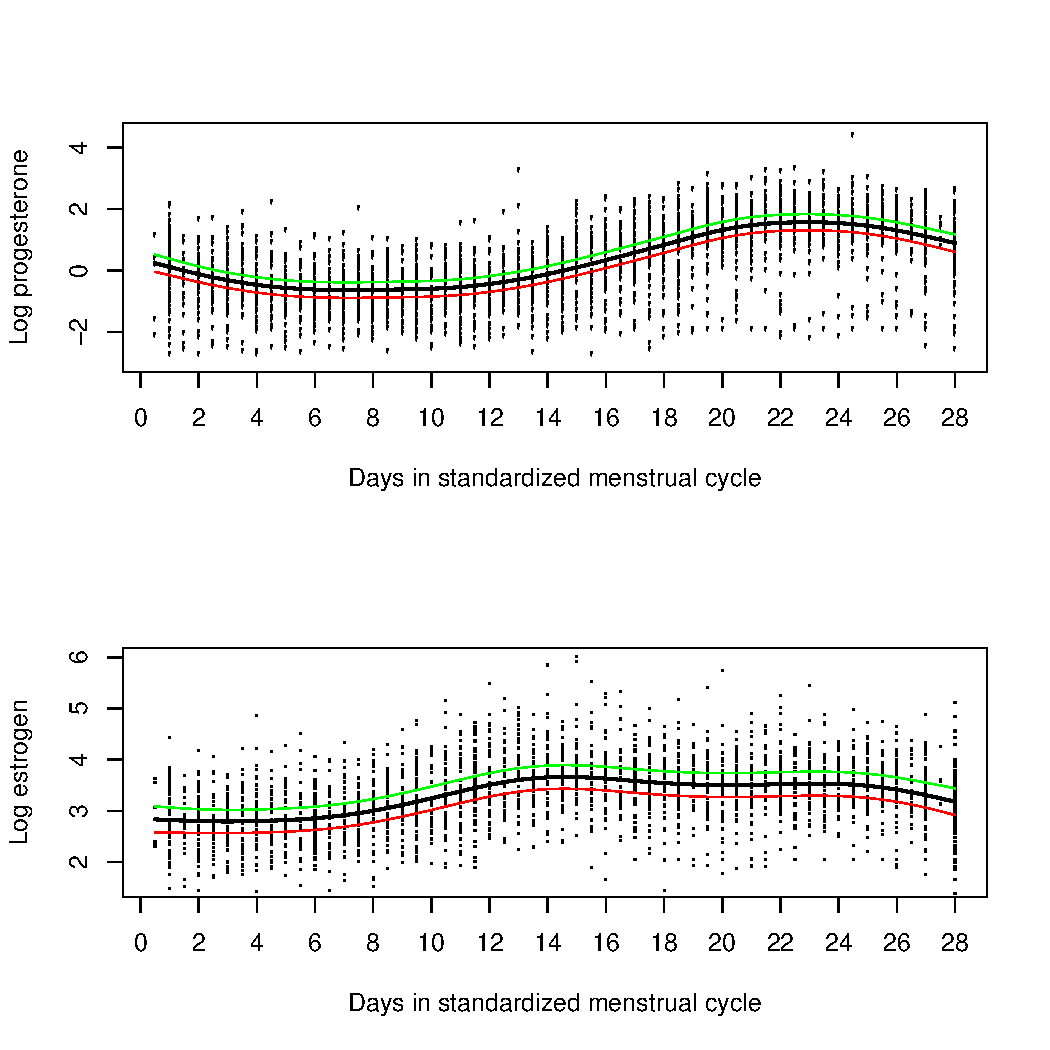
\includegraphics[scale = 0.8]{bivLiuFig1.pdf}
%\caption{Plots of log progesterone  and log estrogen levels against days in a standardized menstrual cycle.}
%\end{center}
%\end{figure}
%
%
%\begin{figure} [h!] \label{Liu2}
%\begin{center}
%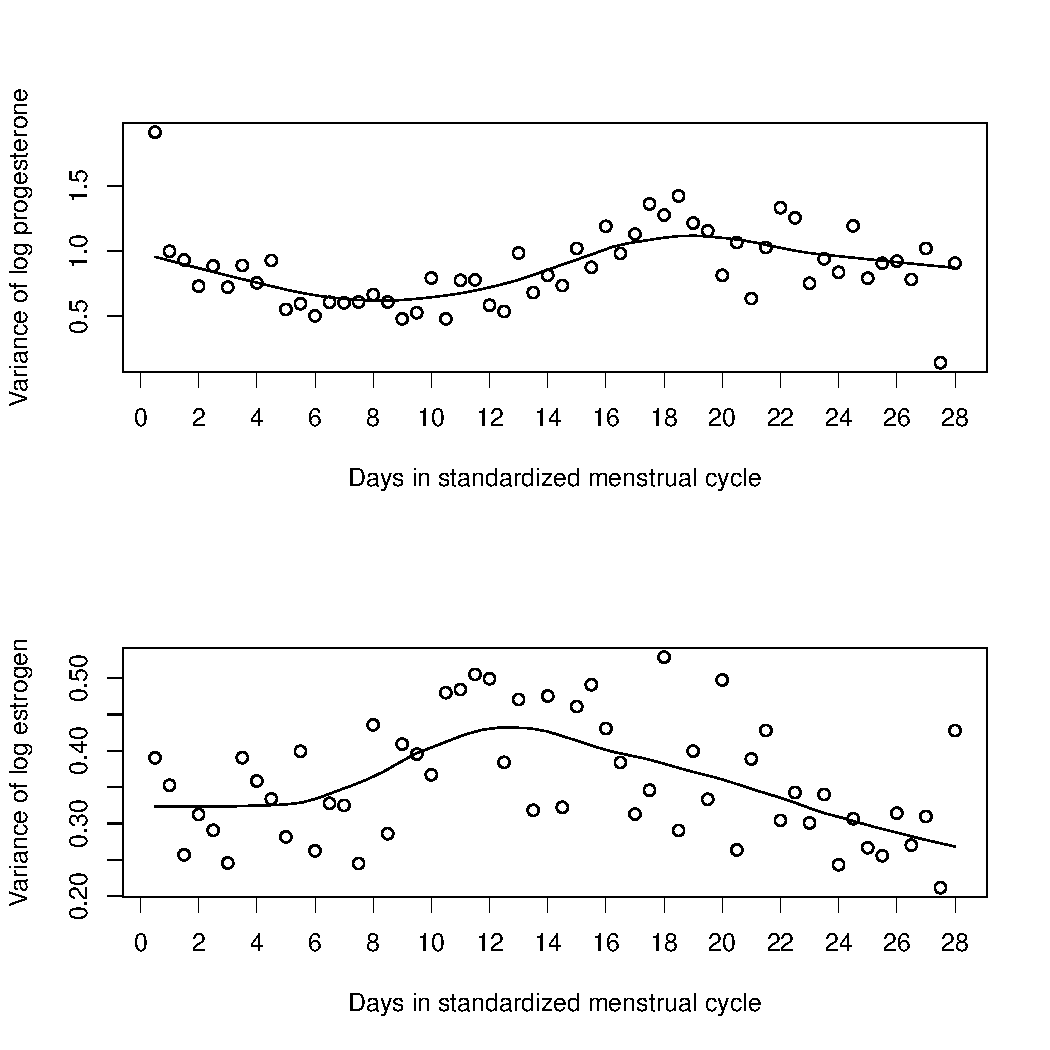
\includegraphics[scale = 0.8]{bivLiuFig2.pdf}
%\caption{Plots of empirical sample variance of log progesterone  and log estrogen levels at each distinct time points in a standardized menstrual cycle.}
%\end{center}
%\end{figure}


Denoting $\{(Y_{1ij}, Y_{2ij})\}$ the $j^{th}$ log-transformed progesterone and estrogen values measured at standardized day $t_{ij}$ since menstruation for the $i^{th}$ woman, we consider the following bivariate semiparametric stochastic mixed model:
\begin{eqnarray*}
Y_{1ij} &=& {\rm age}_i^T  \beta_{11}  + {\rm underWeight}_i^T  \beta_{12}
+ {\rm overWeight}_i^T  \beta_{13}
+ f_1(t_{ij}) + b_{1i} + U_i(t_j) + \epsilon_{1ij} 
 \\
Y_{2ij} &=& {\rm age}_i^T  \beta_{21} +  {\rm underWeight}_i^T  \beta_{22}
+  {\rm overWeight}_i^T  \beta_{23}
+ f_2(t_{ij}) + b_{2i} + U_i(t_j) + \epsilon_{2ij} 
\\
&& i = 1, \dots, 100; j  = 1, \dots, n_i; t_{ij} \in \{0.5, 1.0, \dots, 28\}
\end{eqnarray*}
where $b_{1i}$ and $b_{2i}$ are the random intercepts that are correlated between the two hormone response but independent between subjects following a bivariate normal distribution with mean zero and variance 
$
\begin{pmatrix}
\phi_{1} &   \phi_{3}  \\
\phi_{3} &   \phi_{2} 
\end{pmatrix};
$
%$
%N_2 \left(
%\boldsymbol 0, 
%  \begin{pmatrix}
%  \phi_{1} &   \phi_{3}  \\
% \phi_{3} &   \phi_{2} 
% \end{pmatrix}
%\right)
%$;
the $U_i$ are mean $0$ bivariate Gaussian field modeling serial correlation, and the $ \epsilon_{1ij} $ and $ \epsilon_{2ij}$ are independent mean zero measurement errors following bivariate normal with variance  
$
  \begin{pmatrix}
 \sigma_1^2 & 0  \\
0 &   \sigma_2^2 
 \end{pmatrix}.
$
Covariates underWeight and overWeight are indicator variables. 
For computational stability, standardized days were centered at the median day 14 and divided by 10; covariate age is also centered at median 33 years old and divided by 100. Thus, $f_1(t)$ and $f_2(t)$ represents the progesterone and estrogen curve for women of 33 years old with normal weight. 
%\begin{center}
%\begin{tabular}{l*{6}{c}r}
%\hline
%\hline
%Model parameters              & Parameter estimate   & SE  
%%& Standard Error  
%\\
%\hline
%$\beta_{11}$       & -1.1879         & 2.3285          \\
%$\beta_{12}$       & -0.1048         & 0.3666          \\
%$\beta_{13}$       & -0.2647         & 0.2633          \\
%$\beta_{21}$       & -1.5273         & 2.0618          \\
%$\beta_{22}$       & -0.0860         & 0.3246          \\
%$\beta_{23}$       &  0.0579         & 0.2332          \\
%$\tau_1$   &   5.1481      \\
%$\tau_2$   &   1.8003      \\
%$\phi_1$   &   0.4632      \\
%$\phi_2$   &  -0.1984      \\
%$\phi_3$   &   0.4459      \\
%$\sigma_1^2$   &   0.5474      \\
%$\sigma_2^2$   &   0.4648      \\
%$\rho_1$   &   0.2103      \\
%$a_{10}$   &  -0.4326      \\
%$a_{11}$   &   0.3229      \\
%$a_{12}$   &  -0.2187      \\
%$\rho_2$   &   0.1462      \\
%$a_{20}$   &  -1.5891      \\
%$a_{21}$   &   0.3419      \\
%$a_{22}$   &  -0.0855      \\
%\end{tabular}
%\end{center}



Table \ref{tableLiu} records the results of estimates of regression coefficients, smoothing parameters and variance components. It comes as no surprise that the estimate of age has negative impact on both responses and almost all overweight or underweight also affect  both responses negatively; however, noting the associated standard errors of each estimate, possibly larger than might be expected based on the relatively small sample size of this demonstration analysis, these effects are not statistically meaningful. 
Figure \ref{Liu1} superimposed the estimates of nonparametric function $\hat f_1$ and $\hat f_2$ and their 95\% confidence interval, respectively, which accurately captured the underlying trends of the bivariate longitudinal responses.


%======================================================================
%
% CONCLUSION AND DISCUSSIONS
%
%
%======================================================================

\section{Discussions} \label{conclu}

We propose and build a model for analysis of bivariate cyclic longitudinal data and provide inference procedures. The model is proposed in the likelihood framework and the regression parameters and nonparametric functions are estimated by maximizing a penalized likelihood function.  
The smoothing parameter and variance components are numerically estimated using the Fisher-scoring algorithm based on restricted maximum likelihood.
Modelling the time effect nonparametrically gives more flexibility and the Gaussian field allows for additional flexibility in within-subject correlation structure. Simulation results show that inference procedure performs well in all estimation results.

The model we proposed can also be readily extended to multivariate cyclic longitudinal data.   
Dimensionality can pose as a challenge during the extension however. In the bivariate studies, we employed both C++ and parallel computing in the simulation study. Despite the effort, there is still computational burden to this methodology's estimation. Also, special attention was given to parameter initialization as some initialization of parameters may lead to infinity in some entries of variance-covariance matrix, thus causing the matrix degenerate. This said, in the analysis of the real dataset, we tried three much different initializations of the parameters from one another, and all estimates of the regression parameters, the variance components, and smoothing parameters are qualitatively the same, which is reassuring. 


We would like to further explore sensitivity/robustness to the model assumptions. We have investigated the impact of Gaussian field misspecification in the simulation studies, which show that the choice of Gaussian field has little impact on estimates of parameter of interest. However, if we were interested in the underlying biological process, a deeper understanding of the choice in the Gaussian field is needed. 
In spite of further work to consider, this is a flexible and informative method for modeling bivariate cyclic longitudinal response data and we look forward to further extensions of this work in the above and possibly other directions.


%======================================================================
%
% REFERENCE
%
%
%======================================================================

\begin{thebibliography}{9}
% \expandafter\ifx\csname natexlab\endcsname\relax\def\natexlab#1{#1}\fi

\bibitem[{Brumback \& Rice(1998)}]{Brumback:1998}
Brumback, B.~A. \& Rice, J.~A. (1998).
\newblock {Semiparametric stochastic mixed models for longitudinal data}.
\newblock \textit{Journal of the American Statistical Association} \textbf{93}, 961--976.

\bibitem[{Gold et~al.(1995a)Gold, Eskenazi, Hammond, Lasley, Samuels, O'Neill Rasor, Hines, Overstreet \& Schenker}]{Gold:Eske:Hamm:Lasl:Samu:O'Nei:Hine:Over:Sche:quan:1995}
Gold, E.~B.,  Eskenazi, B., Hammond, S.~K., Lasley, B.~L., Samuels, S.~J., O'Neill Rasor, M.,  et al. (1995).
\newblock {Prospectively assessed menstrual cycle characteristics in female wafer-fabrication and nonfabrication semiconductor employees}.
\newblock \textit{American journal of industrial medicine} \textbf{28}, 799--815.

\bibitem[{Gold et~al.(1995b) Gold, Eskenazi, Lasley, Samuels, O'Neill Rasor, Overstreet \& Schenker}]{Gold:Eske:Lasl:Samu:O'Nei:Over:Sche:quan:1995}
Gold, E.~B., Eskenazi, B., Lasley, B.~L., Samuels, S.~J., O'Neill Rasor, M., Overstreet, J.~W. et al.
  (1995).
\newblock {Epidemiologic methods for prospective assessment of menstrual cycle and reproductive characteristics in female semiconductor workers}.
\newblock \textit{ American journal of industrial medicine} \textbf{28}, 783--797.

\bibitem[{Green(1987)}]{Green:1987}
Green, P.~J. (1987).
\newblock {Penalized likelihood for general semi-parametric regression models}.
\newblock \textit{International Statistical Review} \textbf{55}, 245--260.
 
 \bibitem[{Green \& Silverman(1994)}]{Green:1994}
Green, P.~J. \& Silverman, B.~W. (1994).
\newblock \textit{{Nonparametric Regression and Generalized Linear Models: A roughness penalty approach}}.
\newblock London, UK: Chapman and Hall/CRC.

 \bibitem[{Koralov \& Sinai(2007)}]{Koralov:2007}
Koralov, L.~B. \& Sinai, Y.~G. (2007).
\newblock \textit{{Theory of Probability and Random Processes}}.
\newblock New York, NY: Springer, 2 ed.

\bibitem[{Laird \& Ware(1982)}]{Laird:1982}
Laird, N.~M. \& Ware, J.~H. (1982).
\newblock {Semiparametric regression for periodic longitudinal hormone data from multiple menstrual cycles}.
\newblock \textit{Biometrics} \textbf{38}, 963--974.

\bibitem[{Liang \& Zeger(1986)}]{Liang:1986}
Liang, K.~Y. \& Ware, S.~L. (1986).
\newblock {Longitudinal data analysis using generalized linear models}.
\newblock \textit{Biometrika} \textbf{73}, 13--22.

\bibitem[{Liu et~al.(2014)Liu, Cappola, Crofford \&
  Guo}]{Liu:Capp:Crof:Guo:quan:2014}
Liu, Z., Cappola, A.~R., Crofford, L.~J. \& Guo, W.
  (2014).
\newblock {Modeling bivariate longitudinal hormone profiles by hierarchical state space models}.
\newblock \textit{Journal of the American Statistical Association} \textbf{109}, 108--118.

\bibitem[{Raffa \& Dubin(2015)}]{Raffa:2015}
Raffa, J.~D., \& Dubin, J.~A. (2015).
\newblock {Multivariate longitudinal data analysis with mixed effects hidden Markov models}.
\newblock \textit{Biometrics} \textbf{71}, 821--831.

\bibitem[{Sy, Taylor, \& Cumberland (1997)}]{Sy:Cumb:Tayl:quan:1997}
Sy, J.~P.,  Taylor, J.~M.~G. \& Cumberland, W.~G. (1997).
\newblock {A stochastic model for the analysis of bivariate longitudinal AIDS data}.
\newblock \textit{Biometrics} \textbf{53}, 542--555.

\bibitem[{Taylor et~al.(1994)Taylor, Cumberland \&
  Sy}]{Tayl:Cumb:Sy:quan:1994}
Taylor, J.~M.~G., Cumberland, W.~G. \& Sy, J.~P. (1994).
\newblock {A stochastic model for analysis of longitudinal AIDS data}.
\newblock \textit{Journal of the American Statistical Association} \textbf{89}, 727--736.

\bibitem[{Verbyla et~al.(1999)Verbyla, Cullis, Kenward \&
  Welham}]{Verb:Cull:Kenw:Welh:quan:1999}
Verbyla, A.~P., Cullis, B.~R., Kenward, M.~G. \& Welham, S.~J.
  (1999).
\newblock {The analysis of designed experiments and longitudinal data by using smoothing splines}.
\newblock \textit{Journal of the Royal Statistical Society: Series C (Applied Statistics)} \textbf{48}, 269--311.

\bibitem[{Wang et~al.(2000)Wang, Guo \&
  Brown}]{Wang:Guo:Brow:quan:2000}
Wang, Y., Guo, W. \& Brown, M.~B.
  (2000).
\newblock {Spline smoothing for bivariate data with applications to association between hormones}.
\newblock \textit{Statistica Sinica.} 377--497.

\bibitem[{Welham et~al.(2006)Welham, Cullis, Kenward \&
  Thompson}]{Welh:Cull:Kenw:Thom:quan:2006}
Welham, S.~J., Cullis, B.~R., Kenward, M.~G. \& Thompson, R.
  (2006).
\newblock {The analysis of longitudinal data using mixed model L-splines}.
\newblock \textit{Biometrics} \textbf{62}, 392--401.

\bibitem[{Wood(2006)}]{Wood:2006}
Wood, S. (2006).
\newblock \textit{{Generalized Additive Models: An Introduction with R}}.
\newblock Boca Raton, Florida: Chapman and Hall/CRC.

\bibitem[{Zhang \& Lin(1998)}]{Zhang:1998}
Zhang, D. \& Lin, X. (1998).
\newblock {Semiparametric stochastic mixed models for longitudinal data}.
\newblock \textit{Journal of the American Statistical Association} \textbf{93}, 710--719.

\bibitem[{Zhang et~al.(2000)Zhang, Lin \&
  Sowers}]{Zhan:Lin:Sowe:quan:2000}
Zhang, D., Lin, X. \& Sowers, M. (2000).
\newblock {Semiparametric regression for periodic longitudinal hormone data from multiple menstrual cycles}.
\newblock \textit{Biometrics} \textbf{56}, 31--39.


\end{thebibliography}

\begin{table}
\centering
\caption{Simulation results for estimates of model parameters based on 500 simulation replicates} 
\label{tableSim}
\begin{tabular}{l*{6}{c}r}
\hline
\hline
Model parameters & True Value &  Parameter estimate &  Bias &  SE  & Model SE\\
%& Model-based SE\\
\hline
$\beta_1$   &  1.00     &  0.9987     &  0.0013     & 0.0271   & 0.0267    \\
$\beta_2$   &  0.75     &  0.7496     &  0.0005     & 0.0282    & 0.0267   \\
$\tau_1$   &  1.00     &  0.7478     &  0.2522     & 0.1460      \\
$\tau_2$   &  1.00     &  0.7388     &  0.2612     & 0.1535      \\
$\phi_1$   &  1.00     &  0.9946     &  0.0054     & 0.0895      \\
$\phi_2$   & -0.50     & -0.5019     & -0.0038     & 0.0730      \\
$\phi_3$   &  1.00     &  0.9971     &  0.0029     & 0.0868      \\
$\sigma_1^2$   &  1.00     &  0.9989     &  0.0011     & 0.0173      \\
$\sigma_2^2$   &  1.00     &  0.9994     &  0.0006     & 0.0185      \\
$\rho_1$   &  0.20     &  0.1620     &  0.1900     & 0.1034      \\
$a_{10}$   & -0.44     & -0.4936     & -0.1218     & 0.7143      \\
$a_{11}$   &  0.30     &  0.3530     &  0.1767     & 0.7607      \\
$a_{12}$   & -0.20     & -0.2151     & -0.0755     & 0.1823      \\
$\rho_2$   &  0.15     &  0.1483     &  0.0113     & 0.1531      \\
$a_{20}$   & -1.60     & -1.8383     & -0.1489     & 0.9225      \\
$a_{21}$   &  0.30     &  0.4771     &  0.5903     & 0.6754      \\
$a_{22}$   & -0.10     & -0.1298     & -0.2980     & 0.1187      \\
\hline
\end{tabular}
\end{table}

\begin{figure} 
\centering
%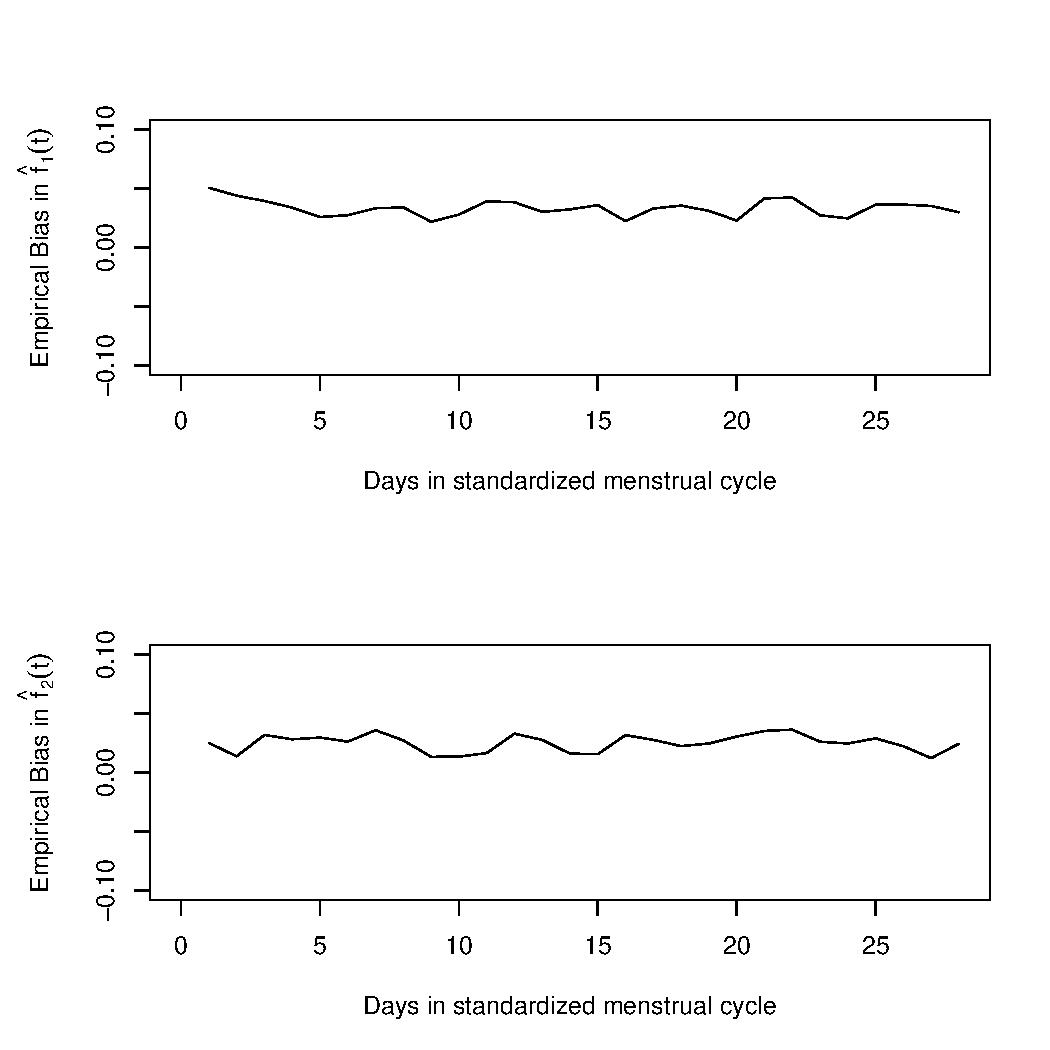
\includegraphics[width=50mm]{bivNOU_liu_Biasf.pdf}
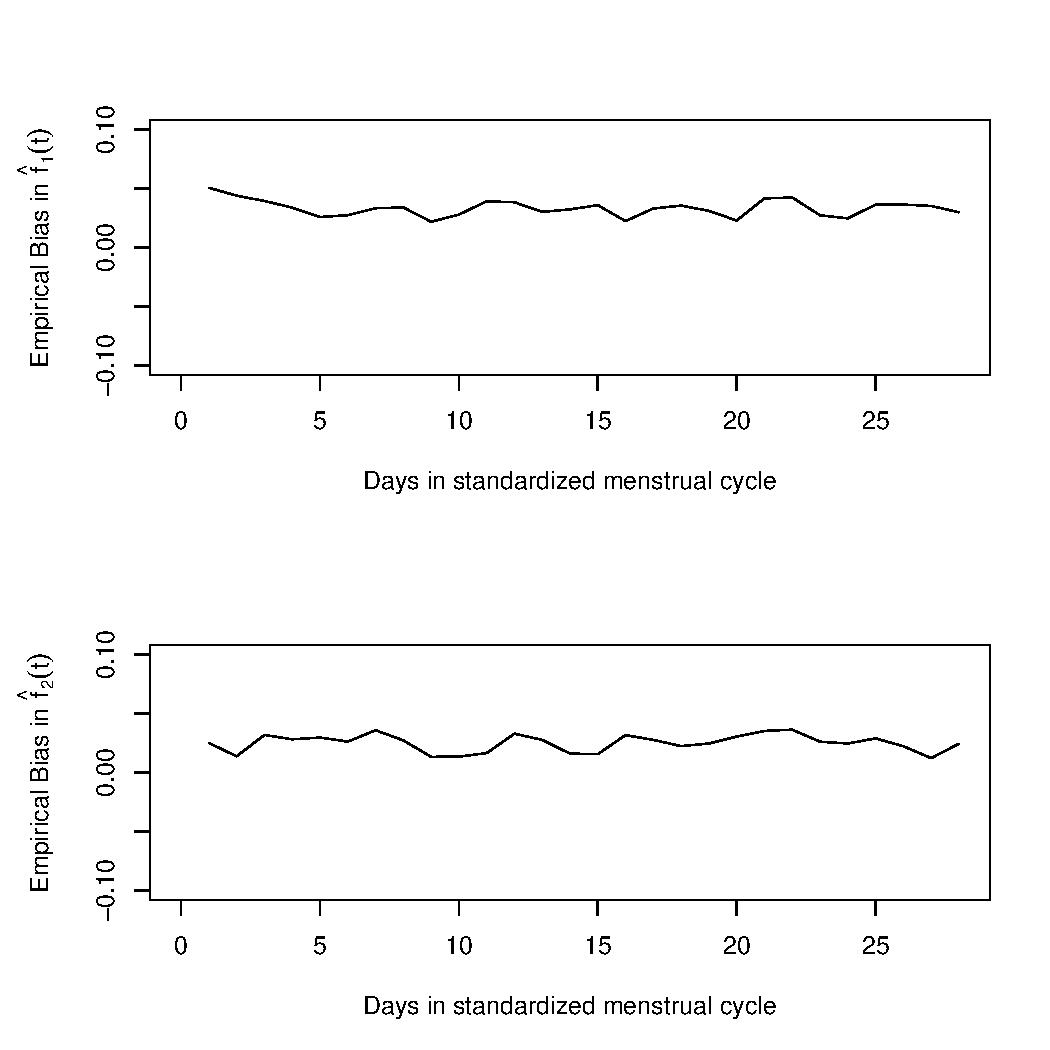
\includegraphics[width=50mm]{bivNOU_liu_Biasf.pdf}
\caption{Empirical Bias in estimated nonparametric functions $\hat f_1$ and $\hat f_2$ based on 500 simulation replications.}
\label{bias}
\end{figure}

\begin{figure} 
\centering
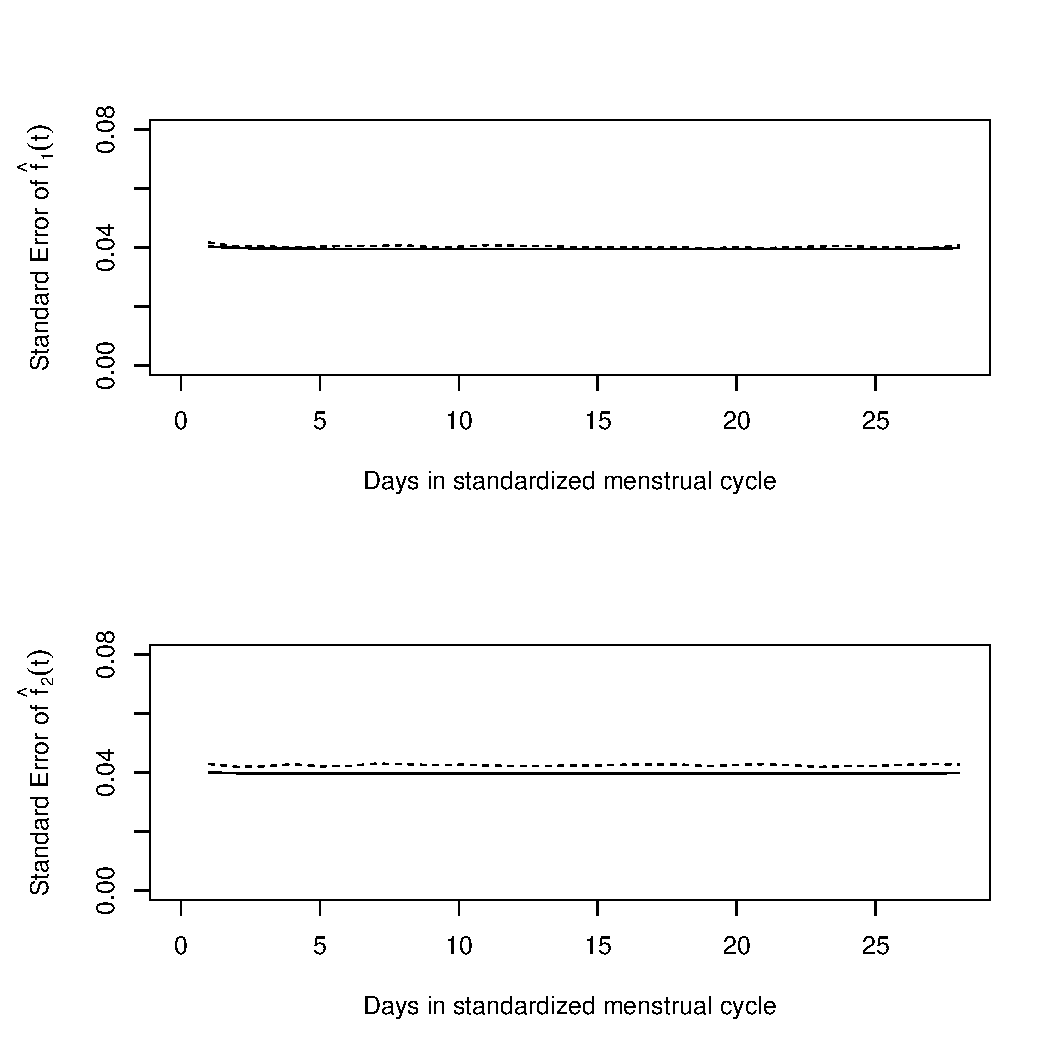
\includegraphics[width=50mm]{bivNOU_liu_SEf.pdf}
\caption{Pointwise empirical (dashes) and frequentist (solid) standard errors of the estimated nonparametric functions $\hat f_1$ and $\hat f_2$ based on 500 simulation replications.}
\label{standarderror}
\end{figure}


\begin{figure}
\centering
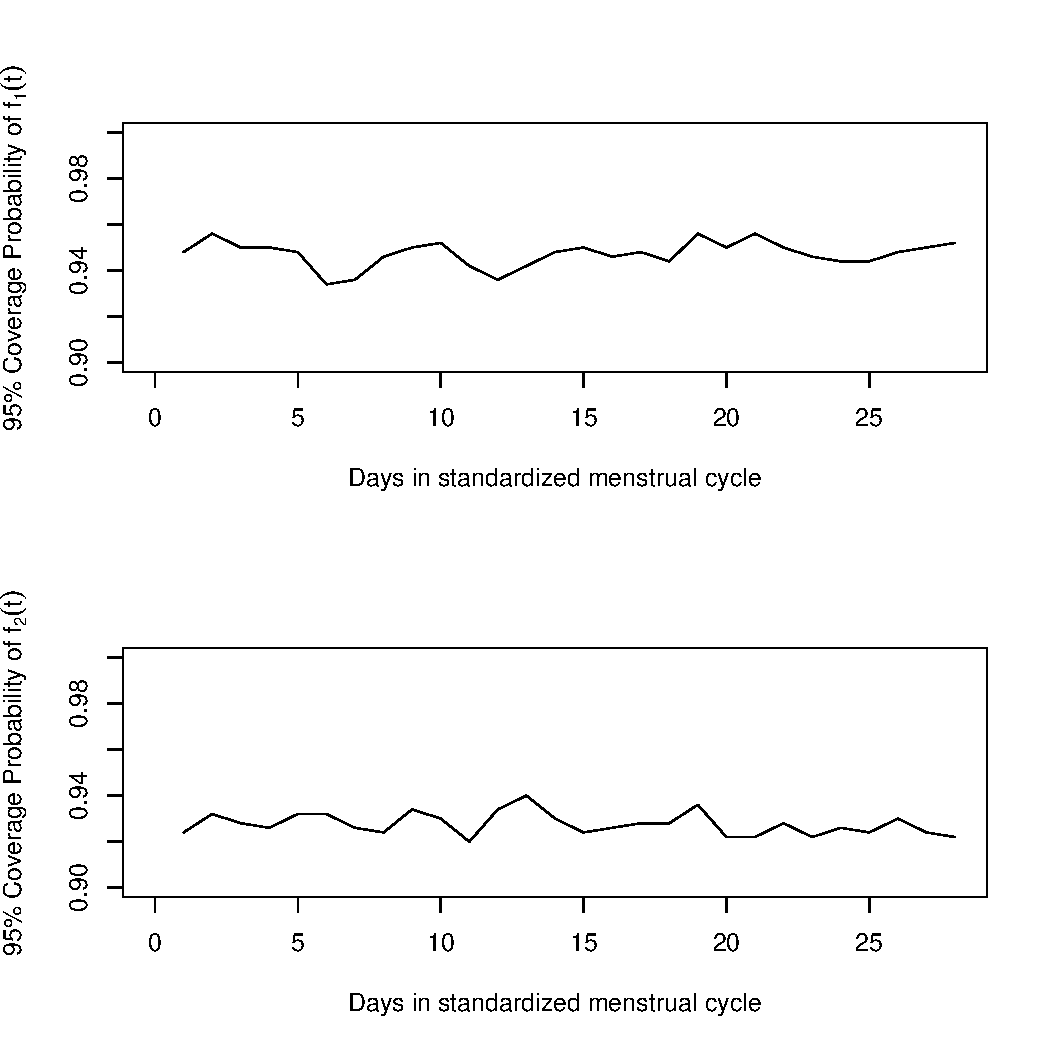
\includegraphics[width=50mm]{bivNOU_liu_cp.pdf}
\caption{A graph showing the estimated 95\% coverage probabilities of the true nonparametric functions $f_1$ and $f_2$ based on 500 simulation replications.}
\label{coverage}
\end{figure}

\begin{table}
\centering
\caption{Estimates of regression coefficients, variance parameter and smoothing parameter for the progesterone and estrogen data.} 
\label{tableLiu}
\begin{tabular}{l*{6}{c}r}
\hline
\hline
Model parameters              & Parameter estimate   & SE  
%& Standard Error  
\\
\hline
$\beta_{11}$       & -1.2651         & 1.8674          \\
$\beta_{12}$       & -0.1687         & 0.2995          \\
$\beta_{13}$       & -0.1837         & 0.2009          \\
$\beta_{21}$        & -0.1455         & 1.7131          \\
$\beta_{22}$        &  0.0068         & 0.2747          \\
$\beta_{23}$        &  0.0765         & 0.1843          \\
$\tau_1$   &   4.6081      \\
$\tau_2$   &   1.8475      \\
$\phi_1$   &   0.6455      \\
$\phi_2$   &  -0.2755      \\
$\phi_3$   &   0.6208      \\
$\sigma_1^2$   &   0.6499      \\
$\sigma_2^2$   &   0.6019      \\
$\rho_1$   &   0.2368      \\
$a_{10}$   &  -0.7699      \\
$a_{11}$   &   0.2894      \\
$a_{12}$   &  -0.1673      \\
$\rho_2$   &   0.0917      \\
$a_{20}$   &  -1.7431      \\
$a_{20}$   &   0.5172      \\
$a_{20}$   &  -0.0800      \\
\hline
\end{tabular}
\end{table}

\begin{figure} 
\centering
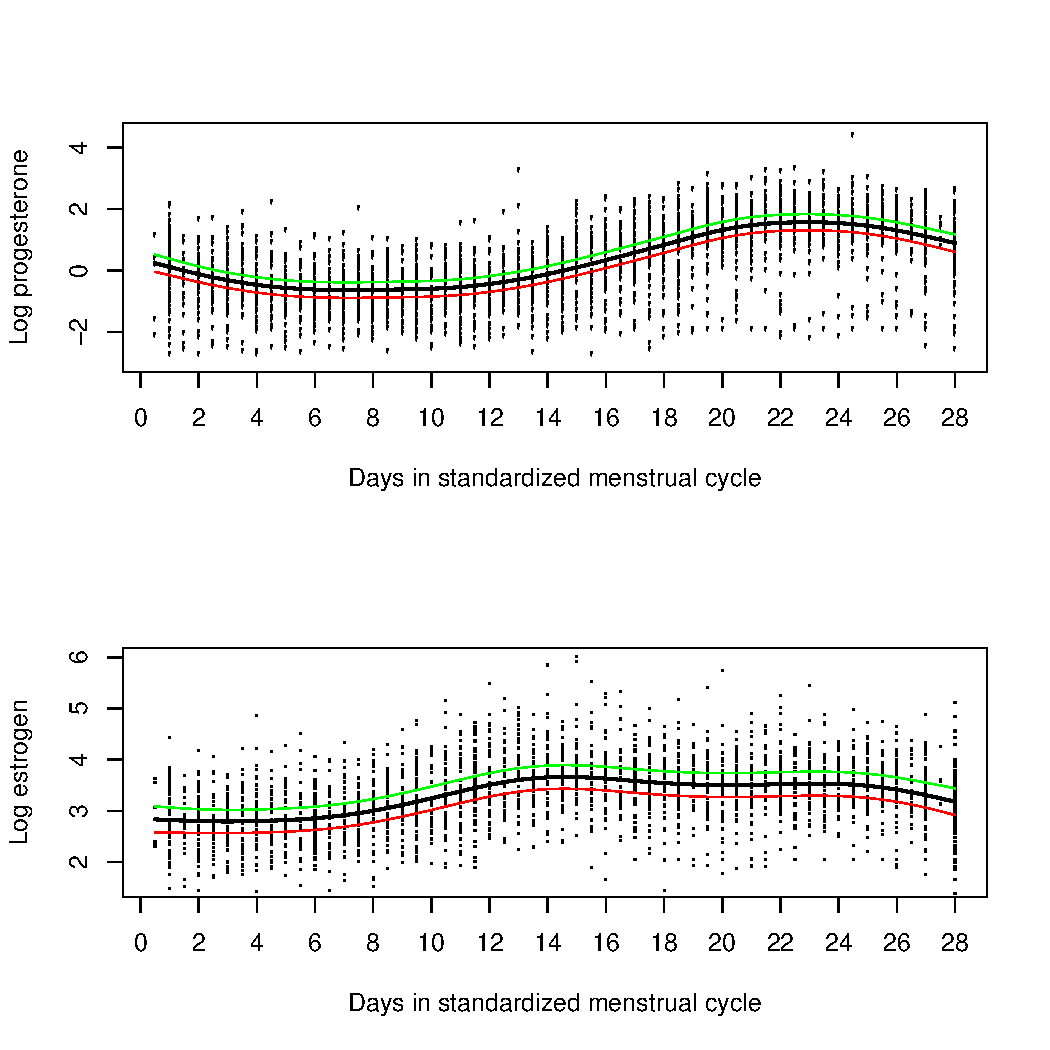
\includegraphics[width=50mm]{bivLiuFig1.pdf}
\caption{Plots of log progesterone  and log estrogen levels against days in a standardized menstrual cycle, superimposed by estimated population mean curve $\hat f_1$ and $\hat f_2$.}
\label{Liu1}
\end{figure}


\begin{figure} 
\centering
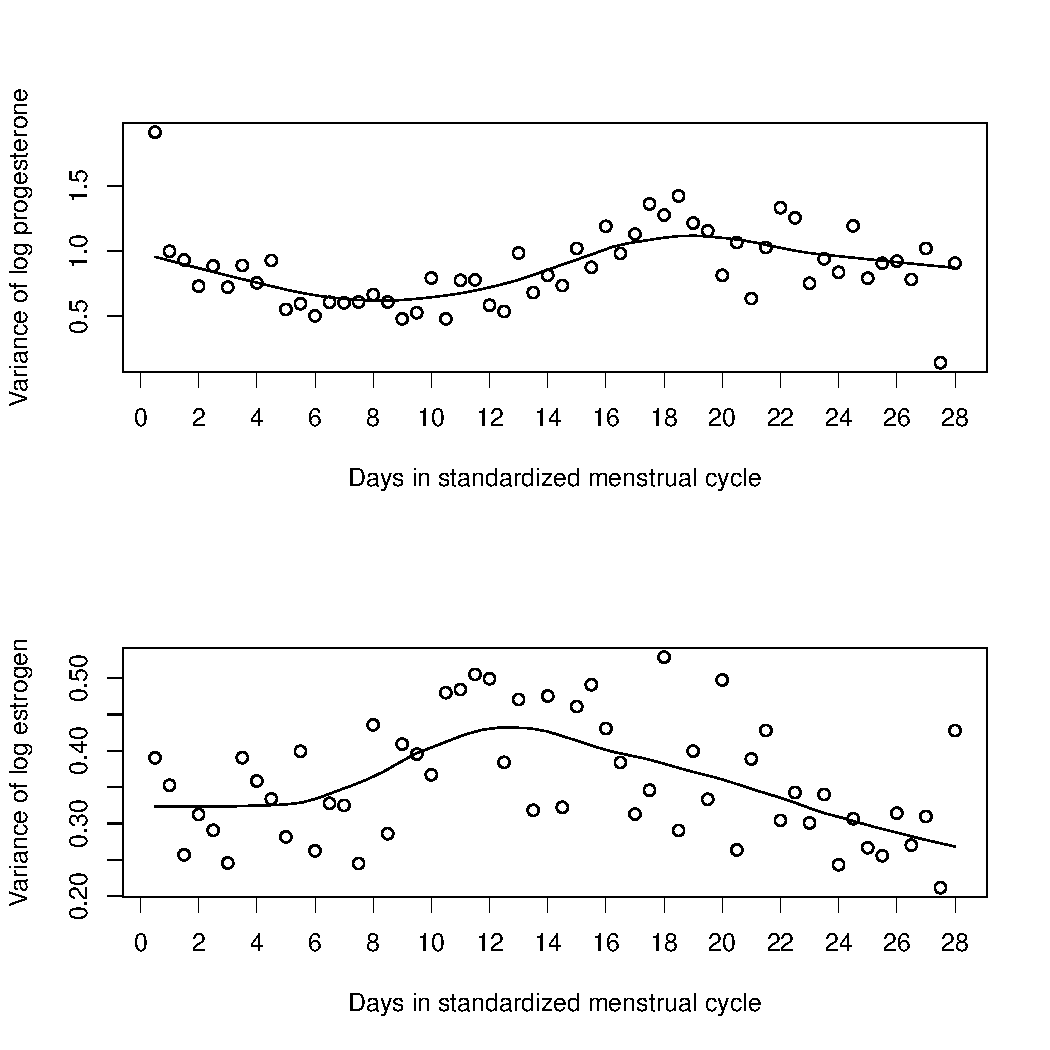
\includegraphics[width=50mm]{bivLiuFig2.pdf}
\caption{Plots of empirical sample variance of log progesterone  and log estrogen levels at each distinct time points in a standardized menstrual cycle.}
\label{Liu2}
\end{figure}

\end{document}
